\documentclass[12pt,oneside,a4paper,chapter=TITLE,section=TITLE,sumario=tradicional,english,brazil]{abntex2}

\usepackage{times}	    		% Usa a fonte Times New Roman
\usepackage[T1]{fontenc}		% Selecao de codigos de fonte.
\usepackage[utf8]{inputenc}		% Codificacao do documento (conversão automática dos acentos)
\usepackage{indentfirst}		    % Indenta o primeiro parágrafo de cada seção.
\usepackage{graphicx}		    	% Inclusão de gráficos
\usepackage{microtype} 		    % para melhorias de justificação
\usepackage{csquotes}
\usepackage{tablefootnote}
\usepackage{amsmath}
\usepackage{pdfpages}
\DeclareUnicodeCharacter{0301}{A-A-A-A-A-}
\usepackage[style=abnt]{biblatex}
\addbibresource{refs.bib}        % Seus arquivos de   % bibliografia vão aqui
%\addbibresource{debug.bib}        % Seus arquivos de   % bibliografia vão aqui
\everymath{\displaystyle}
% ---

\titulo{ANÁLISE DE ESTABILIDADE TRANSITÓRIA UTILIZANDO MÁQUINAS DE APRENDIZADO}
\autor{PABLO MURILO CAPO DE MELO}
\local{CUIABÁ}
\data{2022}
\instituicao{
  UNIVERSIDADE FEDERAL DE MATO GROSSO
  \par
  FACULDADE DE ARQUITETURA, ENGENHARIA E TECNOLOGIA
  \par
  DEPARTAMENTO DE ENGENHARIA ELÉTRICA}
\preambulo{Trabalho Final de Curso apresentado ao Departamento de Engenharia Elétrica da Universidade Federal de Mato Grosso, como requisito parcial para a obtenção do título de Bacharel em Engenharia Elétrica.}
\orientador{Prof. Dr. Carlos Enrique Portugal Poma}
\tipotrabalho{Monografia}

\graphicspath{{figuras/}}
\makeatletter
\hypersetup{
 		pdftitle={\@title}, 
		pdfauthor={\@author},
		colorlinks=true,       		% false: boxed links; true: colored links
    	linkcolor=blue,          	% color of internal links
    	citecolor=blue,        		% color of links to bibliography
    	filecolor=magenta,      		% color of file links
		urlcolor=blue,
		bookmarksdepth=4
}
\makeatother

\renewcommand{\ABNTEXchapterfont}{\fontfamily{\rmdefault}}
\renewcommand{\ABNTEXchapterfontsize}{\normalsize}
\renewcommand{\ABNTEXsectionfontsize}{\normalsize}
\renewcommand{\ABNTEXsubsectionfontsize}{\normalsize}


\makeatletter
\setlength{\@fptop}{5pt} % Set distance from top of page to first float
\makeatother
% ---

% ---
% Possibilita criação de Quadros e Lista de quadros.
% Ver https://github.com/abntex/abntex2/issues/176
%
\newcommand{\quadroname}{Quadro}
\newcommand{\listofquadrosname}{Lista de quadros}

\newfloat[chapter]{quadro}{loq}{\quadroname}
\newlistof{listofquadros}{loq}{\listofquadrosname}
\newlistentry{quadro}{loq}{0}

% configurações para atender às regras da ABNT
\setfloatadjustment{quadro}{\centering}
\counterwithout{quadro}{chapter}
\renewcommand{\cftquadroname}{\quadroname\space} 
\renewcommand*{\cftquadroaftersnum}{\hfill--\hfill}

\setfloatlocations{quadro}{hbtp} % Ver https://github.com/abntex/abntex2/issues/176
% ---

% tamanho do parágrafo
\setlength{\parindent}{1.3cm}
% espaçamento entre um parágrafo e outro
\setlength{\parskip}{0.2cm}  

\makeatletter
\renewcommand{\imprimircapa}{
	\begin{capa}
		\begin{figure}[!h]
   			 \centering
   			 \includegraphics[scale=0.9]{logo_ufmt}
 		 \end{figure}
		\center
		\imprimirinstituicao
	
		\vspace*{1cm}
	
		\imprimirautor
	
		\vfill
		\begin{center}
		\textbf{\imprimirtitulo}
		\end{center}
		\vfill
	
		\imprimirlocal
	
		\imprimirdata
	
		\vspace*{1cm}
	\end{capa}
}
\renewcommand{\imprimirfolhaderosto}{
	\begin{center}
		\imprimirautor
		\vspace*{\fill}\vspace*{\fill}
		\begin{center}
		\textbf{\imprimirtitulo}
		\end{center}
		\vspace*{\fill}
		
		\abntex@ifnotempty{\imprimirpreambulo}{
			\hspace{.45\textwidth}
			\begin{minipage}{.5\textwidth}
				\SingleSpacing
				\imprimirpreambulo
				\vspace*{1cm}
				\par
				\imprimirorientadorRotulo~
				\par				
				\imprimirorientador
			\end{minipage}
			\vspace*{\fill}
		}
		\vspace*{\fill}
		{\imprimirlocal}
		\par
		{\imprimirdata}
	\end{center}
}
\makeatother

% compila o índice
\makeindex

% Início do documento

\begin{document}

\frenchspacing 
\selectlanguage{brazil}
 
\imprimircapa
\imprimirfolhaderosto
\newpage

\begin{folhadeaprovacao}
 \begin{center}
    \imprimirautor

    \vspace*{\fill}\vspace*{\fill}
    \begin{center}
      \textbf{\imprimirtitulo}
    \end{center}
    \vspace*{\fill}
    
    \hspace{.45\textwidth}
    \begin{minipage}{.5\textwidth}
        \imprimirpreambulo
    \end{minipage}%
    \vspace*{\fill}
   \end{center}
   
   \begin{center}
   \textbf{APROVADO PELA BANCA EXAMINADORA}
   \par
   Cuiabá, 15 de dezembro de 2022.
   \vfill
   \textbf{Banca Examinadora:}
   \end{center}
   \assinatura{\textbf{\imprimirorientador \\ Orientador}}
   \assinatura{\textbf{Prof. Dr. Raul Vitor Arantes Monteiro \\ Membro da Banca Examinadora}}
   \assinatura{\textbf{Prof. Dr. Fillipe Matos de Vasconcelos \\ Membro da Banca Examinadora}}
   %\assinatura{\textbf{Professor} \\ Convidado 3}
   %\assinatura{\textbf{Professor} \\ Convidado 4}
      
   \begin{center}
    \vspace*{0.5cm}
    {\imprimirlocal}
    \par
    {\imprimirdata}
    \vspace*{1cm}
  \end{center}
  
\end{folhadeaprovacao}

\noindent
	{Eu, Pablo Murilo Capo de Melo, autorizo o Departamento de Engenharia Elétrica, assim como a Universidade Federal do Mato Grosso, a utilizar e reproduzir meu trabalho, apenas para fins de estudo e pesquisa, sendo expressamente vedado qualquer tipo de reprodução para fins comerciais sem prévia autorização específica do autor.}
	
	\vspace*{1.5cm}
	\assinatura{\textbf{Pablo Murilo Capo de Melo}}
	\vfill
	
\newpage
\begin{agradecimentos}
	Sou muito grato pela oportunidade de ter ingressado na UFMT e mais grato ainda por poder concluir o curso de Engenharia Elétrica na instituição. Agradeço à Deus, minha família, amigos, professores, técnicos  e terceirizados da UFMT e colegas de curso e estágio que me acompanharam durante a graduação. Acredito que sem qualquer um desses que citei, não seria possível chegar onde chegamos.\par
Sou muito feliz por ter conhecido pessoas incríveis neste período, que muito me agregaram e permitiram com que eu seguisse crescendo. Sou mais feliz ainda por saber que, desses muitos, alguns continuarei carregando na minha vida.\par
\end{agradecimentos}

\begin{resumo}
\setlength{\absparsep}{18pt}
	Um sistema elétrico de energia está sujeito a uma série de distúrbios, de diferentes graus de severidade. O mesmo é projetado e operado de forma que fique estável para um dado grupo de contingências, incluindo todos os tipos de curto-circuitos possíveis no sistema. O estudo da estabilidade do sistema elétrico de energia permite predizer o comportamento de tal sistema após uma contingência para quaisquer condições de carga e geração.
O problema da estabilidade transitória em um sistema elétrico de potência gira em torno de manter o equilíbrio no sistema em condições normais e também da capacidade de retornar para tais condições após ser sujeito a um distúrbio transitório severo. A resposta do sistema a um distúrbio transitório severo depende das excursões no ângulo do rotor e da não-linearidade da relação potência-ângulo dos geradores. Ao aplicar-se recursos de aprendizado de máquina para reconhecimento de padrões de simulações do sistema elétrico, é possível inferir sobre a estabilidade do mesmo.
Esta pesquisa busca estudar e avaliar a estabilidade transitória de sistemas elétricos de potência com a utilização de modelos de inteligência computacional baseados em máquinas de aprendizado, apresentando e comparando resultados de aplicação em simulações, bem como resgatando resultados de trabalhos relacionados pré-existentes.

 \textbf{Palavras-chave}: estabilidade transitória. sistemas de energia elétrica. aprendizado de máquina.
\end{resumo}

% resumo em inglês
\begin{resumo}[Abstract]
 \begin{otherlanguage*}{english}
 \setlength{\absparsep}{18pt}
  An electrical energy system is subject to a series of disturbances of differents grades of severity. It is designed and operated in a way that is stable for a given set of contingencies, involving the various types of possible short circuits in the system. The study of the stability of electric power systems allows to predict the behavior of such systems after a contingency for any load and generation conditions.
The problem of transient stability in an electric power system revolves around maintaining equilibrium in the system under normal conditions and also of the ability to return to such conditions after being subjected to a severe transient disorder. The response of the system to a severe transient disturbance depends on the excursions at the rotor angle and the non-linearity of the power-angle ratio of the generators. When applying machine learning resources to recognize patterns of simulation of the electrical system, it is possible to infer about the stability of it.
This research aims to study and evaluate the transient stability of electrical power systems with the use of computational intelligence models based on learning machines, presenting and comparing application results in simulations, as well as retrieving results from related pre-existing works.

   \vspace{\onelineskip}
 
   \noindent 
   \textbf{Keywords}: transient stability. electrical power systems. machine learning.
 \end{otherlanguage*}
\end{resumo}
	
% inserir lista de ilustrações
% ---
\pdfbookmark[0]{\listfigurename}{lof}
\listoffigures*
\cleardoublepage
% ---

% ---
% inserir lista de quadros
% ---
%\pdfbookmark[0]{\listofquadrosname}{loq}
%\listofquadros*
%\cleardoublepage
% ---

% ---
% inserir lista de tabelas
% ---
\pdfbookmark[0]{\listtablename}{lot}
\listoftables*
\cleardoublepage
% ---

% ---
% inserir lista de abreviaturas e siglas
% ---
\begin{siglas}
  \item[API] Interface de Programação de Aplicativos (\textit{Application Programming Interface})
  \item[CA] Corrente Alternada
  \item[CEPEL] Centro de Pesquisas de Energia Elétrica
  \item[CIGRE] Conselho Internacional de Grandes Sistemas Elétricos
  \item[CPU] Unidade Central de Processamento (\textit{Central Processing Unit})
  \item[CVM] Máquina de Vetores de Núcleo (\textit{Core Vector Machine})
  \item[DE] Evolução Diferencial (\textit{Differential Evolution})
  \item[DSA] Avaliação de Segurança Dinâmica (\textit{Dynamic Security Assessment})
  \item[FACTS] Sistema Flexível de Transmissão em Corrente Alternada (\textit{Flexible Alternating Current Transmission System})
  \item[GPU] Unidade de Processamento Gráfico (\textit{Graphics Processing Unit})
  \item[HVDC] Transmissão de Corrente Contínua de Alta Tensão (\textit{High-Voltage Direct Current})
  \item[IEEE] Instituto de Engenheiros Eletricistas e Eletrônicos
  \item[MLP] Perceptron Multicamada (\textit{Multilayer Perceptron})
  \item[OVO] Um Contra Um (\textit{One-Versus-One})
  \item[PMU] Unidade de Medição Sincrofasorial (\textit{Phasor Measurement Unit})
  \item[RAM] Memória de Acesso Aleatório (\textit{Random Access Memory})
  \item[RBF] Função de Base Radial (\textit{Radial Basis Function})
  \item[RFECV] Eliminação Recursiva de Atributos com Validação Cruzada (\textit{Recursive Feature Elimination with Cross-validation})
  \item[RFE] Eliminação de Atributos Recursiva (\textit{Recursive Feature Elimination})
  \item[RNA] Rede Neural Artificial
  \item[SBS] Seleção Sequencial Reversa (\textit{Sequential Backward Selection})
  \item[SCADA] Sistema de Supervisão e Aquisição de Dados (\textit{Supervisory Control and Data Acquisition})
  \item[SFS] Seleção Sequencial Progressiva (\textit{Sequential Forward Selection})
  \item[SGD] Descida Gradiente Estocástico (\textit{Stochastic Gradient Descent})
  \item[SIN] Sistema Interligado Nacional
  \item[SRM] Minimização do Risco Estrutural (\textit{Structural Risk Minimization})
  \item[SVM] Máquina de Vetores de Suporte (\textit{Support Vector Machine})
  \item[UHE] Usina Hidrelétrica
  \item[p.u.] Por Unidade
\end{siglas}
% ---

% ---
% inserir lista de símbolos
% ---
%\begin{simbolos}
 
%\end{simbolos}
% ---

% ---
% inserir o sumario
% ---
\pdfbookmark[0]{\contentsname}{toc}
\tableofcontents*
\cleardoublepage
% ---
\textual
%Introdução
	\chapter{Introdução}
	\section{Considerações Gerais}
De \textcite{kundur2004}, na publicação \textit{Definition and Classification of Power System Stability}\footnote{Definição e Classificação da Estabilidade de Sistemas de Potência} pela \textit{IEEE/CIGRE Joint Task Force on Stability Terms and Definitions}\footnote{Força Tarefa Conjunta IEEE/CIGRE de Termos e Definições em Estabilidade}, nota-se a importância do estudo da estabilidade do sistema elétrico de potência desde os anos de 1920, quando \textit{blackouts} causados por instabilidade tomaram proporções maiores. Nesse aspecto histórico, o fenômeno de instabilidade transitória ganhou a atenção da indústria de energia elétrica no mundo \cite{kundur1994}. De acordo com a evolução dos sistemas elétricos de potência através do aumento de escala e complexidade, do uso de controles e novas tecnologias e a operação constante sob condições intensas de operação surgiu-se diferentes formas de se avaliar a estabilidade de um sistema elétrico, sendo essas: estabilidade do ângulo do rotor, estabilidade de tensão e estabilidade de frequência \cite{kundur1994}.\par
	De acordo com \textcite{kundur2004}, define-se o fenômeno da estabilidade de um sistema elétrico como a capacidade do mesmo, para dada condição inicial de operação, de recuperar um estado equilibrado de operação após ser submetido a um distúrbio físico, de forma que as grandezas elétricas do sistema permaneçam inalteradas. Em \textcite{kundur1994}, aponta-se a estabilidade transitória como a manutenção do sincronismo das máquinas geradoras após serem submetidas a um distúrbio transitório severo, tais como faltas na transmissão, perdas de geração e perdas de carga significativa. A resposta do sistema a tais distúrbios depende das excursões no ângulo do rotor das máquinas geradoras, dependendo, assim, das características não-lineares do sistema elétrico \cite{kundur1994}. \par
	O foco deste trabalho está na discussão da aplicação de modelos de inteligência computacional, baseados em redes neurais artificiais e técnicas de regressão linear, na avaliação da estabilidade transitória de um sistema elétrico de potência, buscando detalhar a construção destes modelos para um caso simulado.\par
	\section{Problemática}
	De \textcite{kundur1994}, o modelo de sistemas elétricos para análise de estabilidade transitória é descrito por um conjunto de equações algébricas e diferenciais não-lineares e possuem diversos métodos de solução. Sendo a integração numérica no domínio do tempo o procedimento padrão de solução, é usada como referência quando comparado a outros métodos.\par
Contudo, como visto em \textcite{swarup2002}, métodos de integração numérica podem demandar um esforço computacional expressivo conforme a complexidade do sistema elétrico aumenta.
Considerando tal cenário, este trabalho busca analisar:
	\begin{itemize}
	\item Quais métodos de solução têm se mostrado mais efetivos para definir a estabilidade transitória de um sistema elétrico de potência?
	\item Quais grandezas elétricas estão envolvidas no fenômeno da estabilidade transitória?
	\item Como é definido o limite de estabilidade transitória do sistema?
	\item Quais as vantagens da utilização das máquinas de aprendizado?
	\end{itemize}
	
	\section{Justificativa}
	A análise de estabilidade transitória se insere no contexto da segurança dinâmica do sistema, sendo um estudo fundamental para garantir que o sistema funcione em equilíbrio, seja em condições normais ou perturbada. 
De forma conjunta com a avaliação de segurança estática, a análise dinâmica é crucial para estabelecer as margens seguras de operação do sistema, bem como para o dimensionamento dos equipamentos elétricos que podem estar presentes como elementos do mesmo.
Considerando o cenário brasileiro de constante expansão energética e a extensão continental do Sistema Interligado Nacional, é fundamental garantir que o sistema elétrico opere em segurança, evitando perdas econômicas e de material para toda a cadeia produtiva ligada ao sistema.
Tendo em mente essa problemática, o estudo e desenvolvimento de ferramentas e métodos aprimorados de análise de estabilidade, tanto dinâmica quanto estática, são muito relevantes para o funcionamento ótimo do Sistema Interligado Nacional.
	\section{Objetivos}
		\subsection{Objetivos Gerais}
		Este trabalho possui como objetivo geral avaliar, no contexto da acurácia dos resultados, o desempenho do modelo de aplicação a ser proposto, verificando a confiabilidade dos métodos baseados em máquinas de aprendizado em constatar a estabilidade ou instabilidade dos sistemas elétricos testados, dadas as condições de distúrbio no sistema em cada caso.
		\subsection{Objetivos Específicos}
		Este trabalho possui como objetivos específicos:
		\begin{itemize}
		\item Comparar as abordagens dos modelos apresentados na revisão bibliográfica;
		\item Explicitar a relevância de tais modelos no âmbito da avaliação de segurança do sistema elétrico de potência;
		\end{itemize}
%Revisão Bibliográfica
\section{Revisão da Bibliografia}
	De acordo com \textcite{haykin1994}, uma rede neural é uma máquina modelada para imitar a forma com que o cérebro humano realiza alguma tarefa, ou seja, uma máquina adaptativa. Destaca-se duas características das redes neurais, que são seu poder computacional e capacidade de generalização. Poder computacional que é entregue através de uma massiva estrutura paralela distribuída e capacidade de generalização devido à habilidade de aprender, que permite obter saídas razoáveis para valores de entrada não-conhecidos \cite{haykin2009}. Ambas características permitem alcançar soluções aproximadas para problemas complexos ou de larga escala que são tradicionalmente intratáveis \cite{haykin2009}.\par
	Muitos trabalhos da literatura trazem a aplicação de redes neurais artificiais na solução do problema da estabilidade transitória de sistemas elétricos de potência, uma vez que métodos convencionais de resolução por integração numérica acabam exigindo muito esforço computacional, à medida que o sistema aumenta seu grau de complexidade \cite{swarup2002}. Métodos convencionais dependem, de acordo com \textcite{paz2004}, das características dos métodos numéricos usados, da complexidade dos modelos matemáticos implementados, da dimensão do sistema elétrico simulado, das constantes de tempo envolvidas, da velocidade do fenômeno simulado, da capacidade do computador e do tempo total de simulação. \par
	De \textcite{haykin2009} e \textcite{haykin1994}, para a aplicação de métodos baseados em redes neurais artificiais, é necessário o treinamento de uma rede neural, que é o processo de aprendizado da máquina, com um conjunto de dados do sistema elétrico de interesse. A composição dos dados contidos no conjunto é então o primeiro objeto de estudo para desenvolver uma rede neural \cite{james2014} capaz de classificar a operação do sistema elétrico de potência quanto a sua estabilidade. \textcite{kundur1994} ao analisar a estabilidade transitória de uma máquina geradora convencional, conclui que existem alguns fatores que contribuem fortemente para o fenômeno, sendo eles:
	\begin{enumerate}
	\item Quão carregado encontra-se o gerador;
	\item Valores de saída do gerador durante a falta;
	\item Tempo de extinção da falta;
	\item Reatância do sistema de transmissão pós-falta;
	\item Reatância do gerador. Uma menor reatância aumenta a potência de pico e reduz o ângulo inicial do rotor;
	\item Inércia do gerador, que influencia no amortecimento da variação do ângulo do rotor, reduzindo a energia cinética adquirida durante a falta;
	\item Tensão interna do gerador, que depende da excitação de campo no rotor;
	\item Tensão do barramento.
	\end{enumerate}
	
	
\textbf{\textit{Kalyani, S., Swarup, K. S., 2011, "Classification and Assessment of Power System Security
Using Multiclass SVM", IEEE Transactions on Systems, Man and Cybernetics.}}\par
	De \textcite{kalyani2011}, um sistema é dito estaticamente seguro se as tensões nas barras e os valores de potência ativa gerada nos barramentos estão dentro dos limites, sem ocorrências de sobrecarga nas linhas. No caso, avalia-se separadamente o equilíbrio do sistema quanto a sua estabilidade de tensão (avaliação de segurança estática) e estabilidade angular (avaliação de segurança transitória). Deseja-se classificar entre quatro níveis de estabilidade, tanto de tensão quanto angular, sendo estes seguro, criticamente seguro, inseguro e altamente inseguro. 
	Para a avaliação de segurança estática, o vetor padrão tem sua composição feita pelos seguintes dados:\par
	\begin{itemize}
\item $|V |_{i}$ - módulo da tensão na barra $i$;
\item $\theta_{i}$ - ângulo da tensão na barra $i$;
\item $S_{G}$ - potência complexa gerada na barra $i$;
\item $S_{Li}$ - potência complexa de carga na barra $i$;
\item $S_{km}$ - fluxo de potência na linha $km$.
	\end{itemize}
	\par
	No caso da avaliação de segurança transitória, o vetor padrão, além de conter as informações obtidas com o fluxo de potência, contém também dados de variáveis dinâmicas do sistema. Compõem o vetor padrão os seguintes dados:\par
	\begin{itemize}
	\item $|V |_{i}$ - módulo da tensão na barra $i$;
	\item $\theta_i$ - ângulo da tensão na barra $i$;
	\item $S_{G}$ - potência complexa gerada na barra $i$;
	\item $S_{Li}$ - potência complexa de carga na barra $i$;
	\item $P{m}$ - potência mecânica injetada na máquina $k$;
	\item $\delta_{0}$ - ângulo do rotor da máquina $k$ no instante de aplicação da falta;
	\item $\delta_{cl}$ - ângulo do rotor da máquina $k$ no instante de remoção da falta;
	\item $\omega_{cl}$ - velocidade do rotor da máquina $k$ no instante de remoção da falta.
	\end{itemize}
	\par 
	Utiliza-se como base de simulação os modelos padrões IEEE de sistema elétrico \textit{New England IEEE 39-bus System} e \textit{IEEE 118-bus System}, em 50Hz, com faixa de segurança de tensão entre 0,90 e 1,10 p.u. nos barramentos. Os dados são retirados de software que, para um universo entre 50\% e 200\% de valores de carga e geração, simula uma falta trifásica com saída de linha única após 12,5 ciclos (0,25 segundo entre a falta e a remoção da linha a 50Hz) em todas as linhas de transmissão, uma por uma. O estado da estabilidade transitória é avaliado através do método de função de energia transitória. Gerou-se 548 e 3537 pontos de operação para os sistemas com 39 e com 118 barras, respectivamente.\par
	Os dados de treinamento dos algoritmos de aprendizagem de máquina passam pela aplicação de algoritmos de seleção sequencial para a seleção de atributos. Em \textcite{theodoridis2003}, caracteriza-se técnicas de seleção de variáveis, tal como o algoritmo de seleção sequencial direta que é utilizado, como uma forma de reduzir a dimensionalidade do problema sem perder a capacidade de generalização do classificador.  \par
	A construção do classificador é baseada em máquina de vetores de suporte, do inglês \textit{Support Vector Machine} (SVM), utilizando \textit{kernel} com função de base radial. Aplica-se uma abordagem que permite a SVM classificar entre quatro classes, ou seja, classificação multinomial ou multiclasse. Visto que a aplicação de SVM inclui apenas uma saída binária, soluciona-se o problema de classificação em multiclasses através da combinação de alguns classificadores SVM binários. Essa combinação é feita através do método OVO - \textit{one-versus-one}, construindo, para o caso, seis classificadores binários. A função decisão da saída do classificador é determinada para todas as combinações de pares de classes \cite{platt2000}\cite{hsu2002}.\par
	 Para a otimização dos parâmetros da SVM, utiliza-se o algoritmo denotado \textit{DE/rand/1/bin} para o processo de evolução diferencial, que consiste na geração de novos vetores de treinamento, chamados de vetores de teste, através de mutação e combinação de vetores padrão aleatórios \cite{storn2005}. No caso, o novo vetor é validado caso satisfaça uma função de adequação pré-definida \cite{storn1997}.\par
	A avaliação dos resultados é feita considerando o processo de redução de dimensionalidade do problema, a acurácia da classificação e a taxa de erro de classificação, em cada uma das quatro classes, para cada um dos dois sistemas elétricos testados. No processo de redução de dimensionalidade do problema, obteve-se  para a avaliação de estabilidade de tensão e transitória os índices de, respectivamente, 11.1\% e 17,7\% para o \textit{New England IEEE 39-bus System} e 9,2\% e 3,8\% para o \textit{IEEE 118-bus System}. Desses valores, portanto, nota-se uma diminuição de eficiência da redução para sistemas mais complexos.\par
	Nos critérios de precisão e taxa de erro, comparou-se a abordagem SVM com outros métodos de aprendizado de máquina para os mesmos sistemas simulados. A abordagem se mostrou superior a esses tanto na fase de treinamento quanto na fase de testes, provando que a abordagem utilizando SVM  é suficiente para a construção de um classificador de alta precisão.\par 
	
	
\textit{\textbf{Edwards, A. R., Chan, K. W., Dunn, R. W., Daniels, A. R, 1996, "Transient Stability Screening Using Artificial Neural Networks Within a Dynamic Security Assessment System", IEE Proceedings - Generation, Transmission and Distribution.}}\par
	O monitoramento \textit{online} do sistema de energia elétrica através de ferramentas de avaliação de estabilidade dinâmica permite que o sistema seja operado o mais próximo dos limites de operação e, consequentemente, permite um controle preciso de geração de energia. Ao se tratar de uma avaliação de segurança em tempo real, destaca-se a velocidade de processamento de métodos de reconhecimento de padrão por redes neurais \cite{xianlin1993}\cite{chan1995}. A abordagem utilizada faz o uso de uma rede neural artificial \textit{feedforward} devido a combinação de sua simplicidade, facilidade de
treinamento e execução on-line não-iterativa rápida \cite{haykin2009}.\par 
	A coleção de dados da abordagem é formada, após as simulações de falta do sistema, a partir das seguintes variáveis:
	\begin{itemize}
	\item Magnitude e ângulo das tensões de fase dos barramentos;
	\item Medidas de potências ativa, reativa e aparente;
	\item Energia cinética das máquinas geradoras;
	\item Ângulo, velocidade e aceleração do rotor;
	\item Momento angular do rotor;
	\item Potência acelerante do rotor;
	\item Erro dos reguladores de tensão;
	\item Tempo estimado para instabilidade assumindo aceleração constante no rotor.
	\end{itemize}
	\par
	Para essas variáveis, se tem uma série de tratamentos possíveis para compor os dados de treinamento, como valor médio e desvio padrão, bem como outras formas estatísticas de se apresentar tais variáveis. Portanto, a coleção dos dados de simulação do sistema elétrico são organizados em sua totalidade através de índices compostos. Essa abordagem permite fácil caracterização e identificação da coleção, otimizando a organização da base de dados de treinamento da rede neural  \cite{pereira2006}. \par
	No trabalho, gerou-se aproximadamente 1900 índices compostos e então utilizou-se de um método de seleção semiautomático para selecionar os índices que se mostram melhores indicadores de estabilidade transitória do sistema. O método consiste em aplicar medidas de correlação estatística, selecionando os dez melhores índices globais para classificação e então treinar a rede neural com a seleção. Os índices individuais tidos como fontes de erros de classificação são eliminados iterativamente até o fim do treinamento. Este procedimento provou que, no caso, 18 índices são suficientes para classificar a estabilidade do sistema elétrico após a falta, obtendo sucesso na redução da dimensionalidade do problema. Desses 18, 14 são relacionados à tensão terminal dos geradores no sistema de potência, mostrando uma forte relação entre tensão terminal e a estabilidade transitória.\par
	O sistema de energia modelado se trata de uma versão reduzida do sistema interconectado nacional do Reino Unido que compreende as regiões norte do País de Gales, norte, centro e sul da Inglaterra e a Escócia e é composto por 100 barramentos e 256 linhas de transmissão. O sistema teve sua topologia alterada, gerando seis cenários de contingência, estes derivados do caso base, que contemplam cenários de aumento de carga, saída de circuito, perda de geração e saída de linha de transmissão.\par 
	Ao todo, foram simuladas 838 contingências, sendo essas falta trifásica com a terra nos barramentos, perdas de carga, perdas de geração e perdas de linhas de transmissão. A rede neural artificial \textit{feedforward} de três camadas foi simulada e configurada para 18 entradas com 10 camadas ocultas de neurônios e um neurônio de saída, obtendo uma precisão acima de 98\% para todos os cenários. Então, conclui-se que o uso de informações estatísticas baseadas num vetor de estado do sistema elétrico é suficiente para determinar a estabilidade pós-falta de um sistema elétrico de potência em um ambiente de monitoramento \textit{online} da estabilidade transitória.\par 
	

\textbf{\textit{Mohammadi, M., Gharehpetian, G. B., 2009, "Application of core vector machines for on-line voltage security assessment using a decision-tree-based feature selection algorithm", IET Generation, Transmission \& Distribution.}}\par
	Apesar dos classificadores baseados em SVM serem superiores aos baseados em redes neurais em termos de precisão e velocidade, para casos com vetores padrão muito grandes sofre por se exceder em tempo e memória \cite{gharehpetian2008}. Isso se deve ao fato de SVMs resolverem problemas de programação quadrática com complexidade de tempo proporcional ao cubo do número de vetores de treinamento do classificador \cite{Burges1998}. Para contornar essa característica, o trabalho propõe a aplicação do algoritmo de aprendizado de máquina CVM - \textit{Core Vector Machine}, inglês para máquina de vetores de núcleo, que combina geometria computacional e o treinamento SVM, com \textit{kernel} de base radial.\par
	O algoritmo CVM reformula o problema de programação quadrática como um problema de menor círculo envolvente, otimizando a solução do SVM ao estabelecer uma aproximação da margem de decisão  pelos vetores chamados \textit{core sets}\footnote{Conjuntos de núcleo}, que contém as mais relevantes variáveis dos vetores suporte para a solução \cite{tsang2005}. Esse método torna o treinamento mais rápido, de complexidade de tempo diretamente proporcional ao número de vetores de treinamento do classificador. De menor dimensão comparado à SVM, possui menor quantidade de vetores de estado do sistema elétrico, pois o número de iterações do treinamento passa a ser dependente apenas do parâmetro usado para realizar a aproximação da margem de decisão \cite{tsang2006}.\par
	A proposta traz quatro níveis de segurança do sistema de energia para a classificação, sendo separados nas classes:
	\begin{itemize}
	\item A - Normal
	\item B - Alerta
	\item C - Emergência Corrigível
	\item D - Emergência Incorrigível
	\end{itemize}
	\par 
	Para as simulações \textit{offline} do sistema em que se deseja avaliar a segurança de tensão, deve-se ter diferentes pontos de operação do sistema e existem diversas formas de se calcular a margem de operação. A forma empregada para delimitar o nível de segurança de tensão é a proposta por \textcite{kessel1986} e se trata do índice \textit{L}, que é uma medida quantitativa para estimar a distância do estado atual do sistema em relação ao seu limite de estabilidade, baseado na solução das equações de fluxo de potência. O índice varia de 0 (condições sem carga) até 1 (colapso de tensão). O maior valor do índice L do sistema define o grau de severidade da contingência simulada e os valores são classificados de acordo com a tabela:\par
	\begin{table}[h]
	\centering
	\caption{Faixa do índice \textit{L} para cada classe}\par 
	\begin{tabular}{c|c} 
	\textbf{Faixa do índice \textit{L}}&\textbf{Classe}\\
 	\hline
 	$0\leq L<0,25$ & A\\
 	$0,25\leq L<0,5$ & B\\
 	$0,5\leq L<0,75$ & C\\
 	$0,75\leq L<1$ & D\\
	\end{tabular}
	\end{table}
	\par
	O processo de seleção de variáveis é destacado pois remover dados desnecessários ou que possam resultar em erro de classificação aumenta a acurácia dos algoritmos de aprendizado de máquina, além de possibilitar análises quanto a qualidade de uma dada variável ao influenciar o resultado da classificação. Isto torna tal processo um dos mais relevantes quanto ao sucesso do classificador \cites{yang1998}{guyon2003}{jensen2001}.\par
	O método empregado para seleção de variáveis se trata da construção de uma árvore de decisão por estimar a aptidão das variáveis para a separação das diferentes classes, além de serem menos computacionalmente intensas em comparação com as redes neurais. A árvore de decisão construída avalia um índice que quantifica a importância de uma variável, de forma que se construa um ranking de variáveis a medida em que a árvore de decisão avança, começando pela mais importante e então decrescendo \cite{breiman1984}. \par
	Durante o processo de seleção de variáveis, reuniu-se ao todo 199 variáveis pela árvore de decisão, sendo essas variáveis referentes as seguintes grandezas elétricas:\par
	\begin{itemize}
	\item Fluxos de potência ativa e reativa;
	\item Tensões nos barramentos;
	\item Cargas ativa e reativa;
	\item Gerações ativa e reativa.
	\end{itemize}
	\par
	O caso estudado se trata do modelo \textit{New England IEEE 39-bus System}, que poussui 10 geradores, 46 linhas e 19 barras de carga. O universo de carga e geração varia de 30\% a 130\% do caso base e resultou em 1375 pontos de operação, sendo 1000 para o treinamento do classificador e 375 para o teste do mesmo. Foram simulados 4 contingências para cada ponto de operação, sendo uma saída de linha única cada e calculou-se o índice \textit{L} em cada situação, classificando os níveis de segurança de tensão. \par
	O desempenho da proposta foi avaliado nos critérios de tempo de treinamento, de número de vetores suporte, de precisão para cada classe e em sua acurácia total. Os resultados foram comparados, para o mesmo caso, com classificadores baseados em SVM, redes neurais artificiais e árvore de decisão. O método CVM apresenta desempenho superior, sendo notáveis as melhorias em tempo e número de vetores suporte ao comparar-se com SVM.\par 
\textbf{\textit{Xu, Y., Zhang, R., Zhao, J., Dong, Z. Y., Wang, D., Yang, H., Wong, K. P., 2016, "Assessing Short-Term Voltage Stability of Electric Power Systems by a Hierarchical Intelligent System", IEEE Transactions on Neural Networks and Learning Systems.}}	\par
	Por \textcite{kundur1994}, o fenômeno de estabilidade de tensão pode ser dividido em curto prazo e longo prazo. A estabilidade de tensão a curto prazo envolve a dinâmica complexa das cargas conectadas ao sistema de energia, tais como motores de indução que, após uma grande perturbação, desaceleram drasticamente e provocam afundamento de tensão ou até mesmo param de funcionar devido ao torque elétrico inferior à carga mecânica do motor. Tais efeitos requerem alta corrente reativa que afeta de forma adversa a magnitude da tensão terminal, correndo risco de colapso após o efeito transitório de tensão \cites{cutsem1998}{diaz2002}.\par
	O modelo matemático do sistema elétrico que inclui a modelagem dinâmica de carga é representado por uma grande coleção de equações diferenciais e algébricas não lineares que são:\par
	\begin{gather}
	\frac{\partial x}{\partial t}=f(x, y, p, \gamma)\\
	0=g(x, y, p,\gamma)
	\end{gather}
\par 
(1.1) corresponde às equações diferenciais dos componentes do sistema, incluindo geradores, motores, cargas dinâmicas, bem como seus sistemas de controle, dentre outros\par 
(1.2) corresponde às equações algébricas da rede e cargas estáticas\par 
De (1.1) e (1.2)\par 
$x$ -- variáveis de estado, como ângulos de geradores e tensões dinâmicas em barra\par 
$y$ --  variáveis algébricas, como tensões e angulo de tensões de cargas estáticas\par 
$p$ -- parâmetros controlados, como controles de sistemas automáticos de regulação de tensão\par
$\gamma$ -- parâmetros não-controláveis, como níveis de carga\par  

Essas equações não podem ser resolvidas analiticamente e são solucionadas por métodos de integração numérica em uma simulação no domínio do tempo. O impacto da dinâmica de carga é o objeto principal de estudo do desempenho da tensão a curto prazo como resposta a distúrbios de diferentes graus de severidade em um sistema de energia que, no caso, se trata do modelo \textit{New England IEEE 39-bus System}. A modelagem dinâmica da carga torna a simulação no domínio do tempo mais próxima do sistema real e, portanto, mais confiável \cite{xu2010}.\par 
O classificador é uma rede neural artificial com pesos aleatórios, que é essencialmente diferente de redes neurais tradicionais, pois a atribuição do peso das entradas é feita de forma aleatória e a atribuição dos pesos de saída é feita através de cálculos de matriz direta. Contudo, a aleatoriedade da atribuição dos pesos torna o método instável pois cada modelo resultante pode ser considerado como uma instância de uma variável aleatória. Portanto, é importante desenvolver um critério para a inicialização do método através de mecanismos supervisão para se obter uma melhor performance \cite{schmidt1992}.\par
Desenvolve-se dois índices para avaliar a estabilidade de tensão a curto prazo, sendo esses o Índice de Colapso de Tensão Transitória e o Índice de Severidade de Tensão Transitória para Desvio Inaceitável de Tensão Dinâmica. O primeiro é um índice binário que indica quando o sistema perde ou não o equilíbrio a curto prazo após uma perturbação. O segundo considera que, após o retorno à margem de equilíbrio, o sistema ainda sofre com níveis inaceitáveis de variação de tensão, como depressão de tensão prolongada e atraso na recuperação da tensão. O grau de severidade no desvio de tensão é refletido pela magnitude da violação de tensão associada ao tempo de duração do desvio. O método para estabelecer o Índice de Severidade de Tensão Transitória para Desvio Inaceitável de Tensão Dinâmica é o proposto por \textcite{schmidt1992}.\par 
O processo de seleção de variáveis é feito de forma automática, removendo variáveis irrelevantes ou redundantes e diminuindo o tamanho total da coleção de dados de treinamento através do algoritmo proposto por \textcite{xu2011}. Essas medidas reduzem e aumentam, respectivamente, o tempo de treinamento e a acurácia. Para o sistema de energia elétrica, o processo pode identificar as variáveis de operação que melhor descrevem as características da segurança dinâmica, provendo informações relevantes para o controle de segurança \cite{xu2011}.\par
Os dados de treinamento foram gerados a partir do fluxo de potência ótimo e simulação no domínio do tempo, e ainda calcula-se o Índice de Severidade de Tensão Transitória para Desvio Inaceitável de Tensão Dinâmica e o índice de Colapso de Tensão Transitória, com 700 diferentes pontos de operação cobrindo níveis de 80\% a 120\% de carga e geração. Aplica-se um curto-circuito trifásico no barramento 15 por 0,2 segundo e para cada condição de operação, escolhe-se, sendo ao todo 199 variáveis candidatas, a composição do vetor de entrada das seguintes coleções:\par 
\begin{enumerate}
\item Carga ativa e reativa, magnitude da tensão e ângulo de tensão de cada barra de carga
\item Geração de potência ativa e reativa de cada gerador
\item Carga e geração total de todo o sistema
\end{enumerate}
\par 
O tempo total da simulação no domínio do tempo é de 5 segundos com um passo de 0,01 segundo e calcula-se o Índice de Colapso de Tensão Transitória e o Índice de Severidade de Tensão Transitória para Desvio Inaceitável de Tensão Dinâmica para cada um dos 700 pontos de operação, sendo 256 casos de colapso de tensão e 444 não. A rede neural é treinada a partir da coleção de dados uma vez em que escolhe-se aleatoriamente 25\% da coleção para usar como teste após o treinamento. \par
O algoritmo utilizado para extração de atributos é denotado RELIEF \cite{zhang2012}, que indica a capacidade de uma determinada variável distinguir as condições de operação em termos de estabilidade de tensão a curto prazo, sendo que um alto valor RELIEF indica alta capacidade \cite{zhang2012}.\par
Para conceber o modelo, construiu-se 100  redes neurais de pesos aleatórios individuais para que, após o treinamento, seja possível aplicação \textit{online}. Os resultados da proposta são comparados com os resultados de outros métodos, sendo esses SVM, árvore de decisão, rede neural com função de base radial e uma única rede neural com pesos aleatórios. O método proposto apresenta acurácia superior e menor erro de predição em relação aos outros, chegando a mais de 99\% de precisão. Conclui-se então que o sistema inteligente proposto é validado para o caso e aumenta a performance de uma rede neural com pesos aleatórios.\par

\textbf{\textit{Swarup, K. S., Corthis, P. B., 2002, "ANN Approach Assesses System Security", IEEE Computer Applications in Power.}}\par
O algoritmo do mapa auto-organizável de Kohonen é utilizado para treinar uma rede neural para classificar a segurança estática de um sistema de energia elétrica. O algoritmo utiliza aprendizagem competitiva, diferente dos algoritmos de retropropagação e gradiente descendente que aprendem por correção de erro, e é treinado de forma não supervisionada. O mapa é uma forma de representação discretizada dos dados de treinamento com redução de dimensionalidade \cite{kohonen1990}.\par
No caso, a classificação da segurança do sistema elétrico de potência é tida entre seguro e inseguro em 4 níveis, sendo esses Normal, Alerta, Emergência Corrigível e Emergência Incorrigível, onde cada um desses representa, respectivamente, <100\%, 100-150\%, 150-200\% e >200\% de carga do caso base. O algoritmo é alimentado com os fluxos de linha dos diversos casos que compõem a coleção de dados de simulação e o mapa de Kohonen é gerado, agrupando os dados baseado nos limites de carga. A saída do algoritmo provê informação sobre a violação da margem de segurança do sistema elétrico, permitindo a classificação.\par 
O sistema elétrico modelado possui 6 barramentos e 11 linhas de transmissão. Os vetores de entrada da rede neural são os fluxos de potência obtidos através de simulação computacional, sendo 11 valores de potência ativa e 11 de potência reativa, formando vetores de entrada de 22 dimensões para cada caso. Ainda, o algoritmo calcula um índice de segurança em que se baseia a classificação da avaliação de segurança do sistema de energia. Gerou-se ao todo 330 padrões de treinamento com a rede neural configurada com 16 neurônios de Kohonen e antes do treinamento, cada neurônio representa uma contingência. Depois do treinamento, as contingências com padrão de valores de carga similares são agrupadas em cada neurônio. O algoritmo também é testado nos sistemas \textit{IEEE 14-bus System}, \textit{IEEE 30-bus System}, \textit{IEEE 118-bus System} e \textit{IEEE 300-bus System}.\par
 O método permite, através da organização do mapa de Kohonen, a mostra de informações valiosas do sistema estudado de forma visual \cite{kohonen1990}. O agrupamento de dados e interpretação dos resultados em uma interface permitem uma clara visualização do estado em tempo real dos componentes do sistema, o que é vantagem para a natureza auto-organizada do mapa.\par 
\textbf{\textit{Huang, S. J., 2001, "Static security assessment of a power system using query-based learning approaches with genetic enhancement ",  IEE Proceedings - Generation, Transmission and Distribution.}}\par
Como forma de melhorar o desempenho de uma rede neural, é proposta a aplicação de aprendizagem baseada em consulta com aprimoramento por algoritmo genético para avaliar a segurança estática do sistema de energia, sendo essencialmente diferente do aprendizado feito a partir de dados gerados aleatoriamente. A proposta requer perguntar à uma rede neural parcialmente treinada para responder a questões e as respostas são levadas a um oráculo, que é responsável por selecionar as variáveis mais informativas e representativas quanto a avaliação de segurança estática do sistema de energia. O oráculo busca então garantir resultados de avaliação, melhorando a qualidade dos dados de treinamento \cite{chang1997}.\par 
O método abordado requer que a rede neural parcialmente treinada tenha uma coleção de pontos de dados inversos, onde avalia-se o gradiente da superfície de decisão multidimensional. Do gradiente, os pontos de consulta são adquiridos por amostragem de pares conjugados, gerando os dados de consulta e então é utilizado para refinar a margem de decisão, o que implica no aumento da precisão da classificação enquanto preserva a qualidade dos dados, pois o refino da margem de decisão melhor demarca a separação das variáveis \cite{huang1996}. Contudo, por aumentar o número de vetores de entrada, acaba por aumentar o tempo de treinamento da rede neural. Todavia, tal aspecto acaba por ser compensado pela aplicação do algoritmo genético, que procura a solução ótima do problema de classificação ao alterar as condições de inicialização da rede neural \cite{huang1995}.\par
O tratamento do problema consiste em gerenciar o sistema de larga escala de forma a separá-lo em subproblemas, formando três partições, sendo essas partição de contingência, partição do sistema e partição de violação termal e de tensão. A tarefa da partição de contingência consiste no algoritmo de ranking de contingência de \textcite{hsu1992}, que formula uma lista de contingências. A tarefa de partição do sistema em subsistemas é, de acordo com \textcite{debs1988}, através da utilização de compensação de barramento limite, que ajusta as injeções de potência entre os subsistemas. Para a tarefa de partição de violação, faz-se a checagem dos limites de operação separadamente.\par 
Na extração de variáveis, o método proposto baseia-se no conceito de que os elementos que compõem os vetores padrão que possuem a maior média de separação entre classes são escolhidos como variáveis chave, de acordo com \textcite{pang1974}. O método é casado com o método Karhunen-Loe, de acordo com o proposto por \textcite{fukunaga1970}, que consiste em extrair informações estatísticas de segunda ordem de atributos para assegurar aos dados uma melhor representatividade do sistema de energia elétrica \cite{duda1973}. O método de extração de atributos baseia-se, então, no grau de segregação estatística entre as duas classes, que leva em consideração a média e a variância de uma variável para determinada classe.\par
Por \cite{linden1989}, a aplicação do algoritmo de inversão da rede neural consiste na geração de novos vetores padrão de entrada a partir de saídas de forma aleatória ao longo da fronteira de classificação. O método computa o erro entre a saída da rede neural e a saída do vetor alvo escolhido aleatoriamente. Esse erro é retro-propagado para a camada de entrada da rede neural e ajusta o vetor alvo de entrada enquanto não ajusta os pesos da rede. Do novo vetor gerado pela inversão, calcula-se o gradiente de contorno para indicar a forma da superfície de fronteira. Dos dados do gradiente, baseia-se o oráculo que, de forma inteligente, seleciona as informações que serão usadas para aprimorar a rede neural, tornando-a informativa e representativa às características intrínsecas do sistema \cite{linden1989}.\par
O modelo de sistema elétrico adotado representa o sistema de potência de Taiwan, que não é interconectado com nenhum outro sistema externo, sendo assim um sistema isolado, faz de suma importância a avaliação de segurança para a indústria do país. O sistema é composto por 16 geradores, 170 barras e 121 linhas de transmissão, das quais escolheu-se apenas as linhas de 345 kV e 161 kV para o estudo. Foram testadas duas contingências, sendo ambas saída de linha única porém em regiões diferentes do sistema e gerou-se cerca de 4000 vetores padrão aleatórios para cada contingência. A coleção de dados do sistema inclui as injeções de potências ativa e reativa, a magnitude tensão em todos os barramentos e os fluxos de potência calculados pelo fluxo de potência ótimo com ajuste para reduzir o custo da energia elétrica. \par 
A rede neural é configurada com 24 neurônios de entrada, 1 neurônio de saída, 5 neurônios escondidos e 0,3 de taxa de aprendizagem e para a segunda contingência, altera-se o número de entradas para 20. A classificação de segurança do sistema de energia é feita entre estável e instável, testando a proposta tanto com o aprendizado baseada em consulta quanto sem, a fim de obter resultados comparativos no que tange ao efeito do método proposto. A forma de avaliação de desempenho da abordagem baseia-se na taxa de precisão de classificação e tempo de treinamento e apresenta resultados positivos. Destaca-se o aumento na precisão da classificação ao aplicar-se o método proposto, somando 4\% de precisão no primeiro caso e 2\% no segundo, alterando para, respectivamente, 97\% e 98\% a taxa de classificação.\par

\textbf{\textit{Paramathma, M. K., Devaraj, D., Reddy B, S., 2016, "Artificial Neural Network based Static Security Assessment Module using PMU Measurements for Smart Grid Application",  International Conference on Emerging Trends in Engineering, Technology and Science.}}\par 
	O ambiente \textit{smart grid}\footnote{Redes elétricas inteligentes}, de acordo com \cite{wang2011}, é robusto para flutuação de carga e resiliente para falhas de linha única que causam \textit{blackouts} ou desligamentos, sendo a avaliação de segurança uma das tarefas maiores de sistemas \textit{smart grid}. Em aplicações práticas, é necessário monitorar o ângulo de fase e magnitude da tensão em várias seções ao longo da rede, o que requer medição sincrofasorial via PMU (\textit{Phasor Measurement Unit}\footnote{Unidade de Medição Sincrofasorial}) e que tem como característica obter medição também de toda a vizinhança em que está instalada a unidade de medição \cite{ghosa2013}. Contudo, o alto custo de unidades de medição sincrofasorial torna inviável instalação ao longo de toda a rede elétrica, tornando necessário determinar o posicionamento ótimo das unidades empregando metodologias de algoritmos matemático e heurístico  \cite{aminifar2010}. De acordo com \textcite{paramathma2019} o posicionamento ótimo é tal que possui um número mínimo de unidades de medição sincrofasorial ao mesmo tempo que torna observável todos os nós do sistema de energia.\par
	A proposta consiste em desenvolver um sistema de avaliação de segurança em tempo real utilizando medições sincrofasoriais. O procedimento é dividido em conduzir uma análise de contingência detalhada de eventos severos e/ou inesperados, definir o número e posicionamento ótimo dos PMU com observabilidade completa do sistema através de aplicação de algoritmo genético e avaliar em tempo real a segurança estática utilizando rede neural artificial através de módulo com PMU. \par
	O sistema elétrico testado é o \textit{IEEE 30-bus System}, contendo 24 barras de carga, 6 barras de geração e 41 linhas de transmissão. Os universos de carga e geração variam entre 75\% e 125\% do caso base sob estado de contingência multilinha e para cada caso calcula-se um índice de segurança. Aproximadamente 1000 pares de entrada-saída baseando-se em 750 vetores padrão de treinamento, enquanto 250 vetores para teste, foram gerados para várias saídas de linha única.\par 
	Para a tarefa de classificação, utiliza-se uma rede neural \textit{feedforward} multicamadas de 20 entradas com 3 camadas, das quais 1 é escondida. O treinamento foi feito baseando se nos valores de potências ativa e reativa geradas, potências ativa e reativa de carga e módulo e fase de tensão dos barramentos através do algoritmo de retro-propagação Levenberg-Marquardt pela sua propriedade de convergência \cite{devaraj2007}. A abordagem é validada ao comparar os resultados com cálculo por integração numérica, obtendo resultados satisfatórios. \par 

\textbf{\textit{Jensen, C. A., El-Sharkawi, M. A., Marks, R. J., 2001, "Power System Security Assessment Using Neural Networks: Feature Selection Using Fisher Discrimination", IEEE Transactions on Power Systems.}}\par 
	Em sistemas elétricos de potência, contingências podem incluir perda repentina e inesperada de algum dos circuitos de transmissão ou carga. Tais eventos podem levar a interrupção do serviço em parte ou totalidade do sistema de energia. Portanto, ao avaliar a segurança de um sistema, tem-se o objetivo de determinar quando interrupções de algum serviço é provável de se ocorrer e atuar na redução do risco da contingência.\par 
	O problema de extração de variáveis é tratado pelo discriminante linear de Fisher, que permite ranquear a adequação das variáveis para a avaliação de segurança do sistema de energia elétrica. O método é o proposto por \textcite{weerasooriya1991}, que busca encontrar a função discriminante linear ótimo para a separação das classes estável e instável com base em medidas de correlação estatística. Porém, por se tratar de um método de separação linear, é ineficiente para separações não-lineares. Para a seleção das variáveis, em conjunto com o descrito, utiliza-se uma combinação de algoritmos de seleção sequencial bidirecional e foram selecionadas as 4 melhores para a classificação. Ainda, destaca-se a capacidade do método de ser geral para diferentes topologias do sistema de energia elétrica.\par
	A abordagem é testada no \textit{IEEE 50-generator System}, composto por 50 geradores, 145 barras e 453 linhas de transmissão. A base de dados é gerada a partir de simulação computacional de faltas trifásicas em 9 barramentos diferentes do sistema, sendo essas escolhidas para cobrir uma maior seção do sistema, para 651 pontos de operação diferentes. A rede neural é configurada com 3 camadas e 4 entradas, 10 neurônios escondidos e uma única saída. Para cada uma das 9 faltas, 1000 combinações aleatórias de 4 variáveis foram geradas. O treinamento é feito com cada uma das 1000 combinações. Ainda, utiliza-se a desigualdade de Chebyshev para avaliar a probabilidade de existir combinações melhores que as selecionadas ao delimitar um intervalo de confiança \cites{larson1982}{leon2008}.\par
	O método de discriminação de Fisherman com a abordagem proposta é testado para uma mudança na topologia do sistema e obteve resultado satisfatório ao reduzir a magnitude do erro de classificação geral para o caso. Também é validado para o caso original, constatando a eficiência da análise estatística para a resolução do problema de estabilidade estudado.\par

\textbf{\textit{Amjady, N., 2004, "A Framework of Reliability Assessment With Consideration Effect of Transient and Voltage Stabilities ",  IEEE Transactions on Power Systems.}}\par
A confiabilidade do sistema elétrico, ou seja, a capacidade do sistema elétrico em realizar a própria função, gira em torno de adequação e segurança. Adequação se trata da existência de instalações suficientes dentro da rede para satisfazer a demanda de carga e, por se tratar de condições estáticas, não inclui perturbações no sistema. Já segurança associa-se à resposta do sistema a qualquer perturbação que possa ocorrer \cite{billinton1996}.\par 
	De \cite{amjady1999}, destaca-se a capacidade de generalização de redes neurais e rede neurais \textit{fuzzy}\footnote{Difusas}, sendo essa a característica mais relevante para o sistema de índices compostos inteligentes que é proposto, pois a abordagem pretende considerar adequação e segurança de forma integrada para a avaliação de segurança. O método calcula a adequação baseada em índices de confiabilidade. A avaliação é executada por duas redes neurais \textit{fuzzy} em paralelo, sendo uma responsável pela estabilidade transitória e outra pela estabilidade estática, enquanto uma terceira analisa as características de geração e transmissão para estimar a probabilidade de contingências em estabilidade transitória e de tensão \cite{amjady1999}.\par 
	Da simulação no domínio do tempo, calcula-se as velocidades e aceleração do ângulo do rotor para três intervalos de tempo, sendo esses no instante de extinção da falta, no instante de extinção da falta mais 3 ciclos e depois, mais 6 ciclos. No total, constituem o vetor de entrada da rede neural \textit{fuzzy} as medições de velocidade e aceleração e de tensão para os intervalos descritos. Para a redução da dimensionalidade, aplica-se o conceito de centro de inércia para o sistema de energia.\par 
	Já para a estabilidade de tensão, as variáveis de entrada são dados de tensões em quadratura nos geradores, variáveis mecânicas do rotor nos geradores, estado de carga, reguladores de tensão e transformadores de tap variável para modelagem dinâmica \cite{chowdhury2001}.\par 
	Para seleção de variáveis, utiliza-se o método de análise local, que começa pelo ponto de operação pré-falta até pós pelo conceito de distância elétrica em \cite{amjady2007}. Cada índice de contingência para os diversos casos passa a ter seu vetor de entrada ótimo, garantindo otimização do método. \par 

\textbf{\textit{Sunita, R., Kumar, R. S., Mathew, A. T., 2013, "Online Static Security Assessment Module Using Artificial Neural Networks", IEEE Transactions on Power Systems.}}\par
	Se deseja desenvolver um módulo online de avaliação de segurança estática. A abordagem utiliza um índice composto de segurança para rápida e precisa avaliação de segurança. O módulo computa o índice de segurança para dada condição de operação e provê o status de segurança do sistema, computa o índice de segurança para cada possível condição de saída de linha e identifica contingências tidas como crítica e então, um ranking de contingência é construído baseado nos índices de segurança.\par 
	O índice composto de segurança é construído com base nos fluxos de linha e nas violações dos limites de segurança, usado para classificação do estado de segurança, triagem e ranking de contingência \textit{online}. Define-se dois limites, sendo esses limite de segurança, que é o máximo limite especificado para as grandezas da base de dados, e limite de alarme, que é uma zona adjacente à zona do limite de segurança que indica a proximidade entre elas, em ranking numérico \cite{sunitha2011}.\par
	Os dados de entrada são o as potências ativa e reativa garadas, potências ativa e reativa de carga, magnitude e ângulo de fase das tensões de todos os pontos de operação. Utiliza-se dois tipos de algoritmos, sendo esses redes neurais artificiais \textit{feedforward} multicamada e de função de base radial. A primeira é treinada com o algoritmo de retro-propagação Levenberg-Marquardt devido a sua característica de convergência e \cite{sidhu2000}. A segunda tem por vantagem o mapeamento não linear das variáveis de entrada na saída.\par 
	Se tem que o modelo de teste da abordagem é o \textit{IEEE 118-bus System}, composto por 54 geradores, 118 barras e 177 linhas de transmissão. e são consideradas das contingências possíveis apenas as saídas de linha, variando o universo de carga entre 50\% e 150\% do caso base. Para cada condição de operação, calcula-se o fluxo de potência para as condições de pré e pós-falta através do método de Newton-Raphson. Ao todo, gerou-se aproximadamente 5000 conjuntos de treinamento para 20 contingências aleatórias.\par 
	O desempenho do método é avaliado em comparação com a análise de fluxo de potência por Newton-Raphson, sendo referência, que demanda alto esforço computacional. Disso, os métodos baseados em inteligência computacional se garantem muito mais rápidos de convergir e possuem resultados próximos o suficiente do calculado numericamente. Dos algoritmos, a rede \textit{feedforward} de função de base radial se mostra mais precisa nos resultados em relação à rede neural \textit{feedforward} multicamada devido à sua característica de mapeamento não linear. Dado isso, o módulo é validado para o sistema de potência testado.\par 

\textbf{\textit{Zhang, H., Shen, S., Shen, Y., 2021, "Power System Transient Stability Evaluation Based on Multilayer Perceptron Neural Network", 2021 China Automation Congress (CAC).}}\par
	Inserindo-se em topologias mais atuais, nas quais há presença de um crescente volume de geradores distribuídos ao longo da rede elétrica, no contexto de redes inteligentes, novas metodologias de análise e inferência são desenvolvidas. Ao considerar-se fontes renováveis como turbinas eólicas e geradores fotovoltaicos, o cenário de balanceamento de suprimento e demanda de energia elétrica se torna incerto, dadas características de tais fontes de variarem de forma considerável em diferentes escalas de tempo \cite{schafer2015}. A análise da estabilidade transitória, para um sistema de potência com essas características, é orientada ao comportamento do sistema em cenários de falta de injeções de potência em diversos pontos da topologia \cite{schafer2015}. \par
	Em \textcite{schafer2015}, propõe-se uma metodologia de operação descentralizada de redes  inteligentes, que atrela a atribuição do preço da energia elétrica com a disponibilidade da mesma para dado consumidor de forma descentralizada, encorajando-o a consumir mais em momentos de maior geração de energia como um fator que favorece a estabilização do sistema elétrico. Esta abordagem é usado como base para a construção do sistema-modelo de estabilidade em \cite{arzamasov2018}. Denominado \textit{Decentralized Smart Grid Control}\footnote{Controle Descentralizado de Redes Inteligentes} (DSGC), o modelo assume algumas simplificações para a construção de diversos casos de simulação do sistema elétrico, considerando os geradores como todos de massa rotativa, havendo momento de inércia atrelado ao gerador, e as cargas, todas como massas rotativas síncronas. Além disso, também descarta a presença de controles ativos presentes em linhas de transmissão, como compensadores síncronos estáticos. \par
	O sistema utilizado no trabalho é do tipo estrela com 4 barramentos, sendo um barramento central com outros três em vizinhança, e o conjunto de dados de estabilidade provenientes de \textcite{arzamasov2018} sob domínio da Universidade da Califórnia, Irvine\footnote{Disponível em: \url{<https://archive.ics.uci.edu/ml/datasets/Electrical+Grid+Stability+Simulated+Data+\#>}}. O conjunto de dados possui 10.000 amostras simuladas de pontos de operação da topologia, contando com 12 atributos de entrada e 2 atributos categóricos. Os 12 atributos de entrada são compostos por 11 atributos preditivos e 1 não-preditivo:\par
\begin{itemize}
	\item $T_{x}$: tempo de reação das ações dos dispositivos de controle de estabilidade de frequência;
	\item $P_{x}$: potência nominal, sendo $P_{1}=P_{2}+P_{3}+P_{4}$ onde valores positivos de $P$ representam injeções de potência e negativos, consumo;
	\item $G_{x}$: coeficiente proporcional à elasticidade do preço da energia elétrica;
\end{itemize}
sendo $x=[1, 2, 3, 4]$ representando cada barramento da topologia, onde $x=1$ referente ao barramento de geração central. Os atributos categóricos são referentes à classificação de estabilidade transitória, sendo um índice de estabilidade e uma etiqueta categórica separando casos estáveis e instáveis.\par
O método utilizado na construção do classificador de estabilidade transitória consiste na construção de um grupo de 10 redes neurais multicamadas, de forma que a função decisão do classificador considere contribuições individuais das mesmas. Cada rede neural multicamada tem seu número de neurônios e taxa de aprendizado arbitrados aleatoriamente, de forma que cada uma seja construída como única e posteriormente agregadas como um mesmo classificador.\par 
Os dados de entrada da rede neural são processados pro algoritmo de análise de componente principal para redução de dimensionalidade e a saída é dada por uma estratégia de integração de votação, considerando a saída de cada uma das 10 redes neurais multicamadas construídas no modelo. Essa estratégia, segundo \textcite{zhang2021}, permite com que se obtenha melhores resultados ao se trabalhar com conjuntos de dados desbalanceados, ou seja, quando se há um volume consideravelmente maior de casos estáveis ou instáveis em relação ao oposto.\par 
Os resultados são avaliados considerando métricas definidas, relacionando a capacidade do classificador de se obterem saídas Verdadeiro-Positivo (VP), Falso-Positivo (FP), Verdadeiro-Negativo (VN) e Falso-Negativo (FN), dadas por uma matriz denominada matriz de confusão. As métricas são dadas pelo seguinte:
\begin{itemize}
\item Sensibilidade: $VP/(VP+FN)$, habilidade de reconhecer amostras positivas;
\item Precisão: $VP/(VP+FP)$, proporção de predições verdadeiras em relação ao total de amostras verdadeiras;
\item F-score: $2*VP/(2*VP+FP+FN)$, média harmônica da sensibilidade e da taxa de precisão;
\item Acurácia: $VP+VN/(VP+VN+FP+FN)$, proporção de predições corretas do modelo em relação ao número total de amostras.
\end{itemize}
\par
\section{Resumo dos Trabalhos}
\begin{figure}[ht!]
\centering
\caption{Relação de Tipo dos Classificadores}
\par
\includegraphics[scale=.75]{revisao_classificadores.png}
\centering
\par
FONTE: DE AUTORIA PRÓPRIA
\end{figure}
Considerando quanto ao tipo de classificador utilizado nos trabalhos previamente apresentados, apenas \textcite{kalyani2011}, \textcite{Gharehpetian2009} e \textcite{amjady2004} não utilizam de redes neurais artificiais para a tarefa de classificação, sendo SVM\footnote{Support Vector Machine - Máquina de Vetor de Suporte}, CVM\footnote{Core Vector Machine - Máquina de Vetor de Núcleo}  e RNF\footnote{Rede Neural \textit{Fuzzy}}, respectivamente. A relação dos tipos observados pode ser observada na Figura 1.\par
Contudo, existem diversas formas de construir um classificador de estabilidade com outras técnicas de aprendizagem de máquina, se tratando de um campo de amplo e em constante desenvolvimento.\par

\begin{figure}[ht!]
\centering
\caption{Relação dos Algoritmos de Treino dos Modelos de Aprendizagem de Máquina}
\par
\includegraphics[scale=1]{revisao_treinamento.png}
\centering
\par
FONTE: DE AUTORIA PRÓPRIA
\end{figure}
\par
 Existem outras tendências na comunidade científica, como por exemplo o uso de redes neurais convolucionais (CNN\footnote{Convolutional Neural Networks}), memória de longo curto prazo \cite{lstm} (LSTM\footnote{Long-Short Term Memory}) e técnicas de aprendizado profundo e \textit{Big Data}, observados em \textcite{Hu2017} e \textcite{Han2021}. A Tabela 2 relaciona as Figuras 1 e 2.
\par
\begin{table}[!ht]
    \centering
    \caption{Relação de Classificadores}
    \begin{tabular}{c|c|c}
        \textbf{Publicação} & \textbf{Classificador} & \textbf{Treinamento} \\ \hline
        \textbf{\Cite{kalyani2011}} & SVM & Um Contra Um \\ 
        \textbf{\Cite{Edwards1996}} & RNA & Retropropagação \\ 
        \textbf{\Cite{Gharehpetian2009}} & CVM & Regressão \\ 
        \textbf{\Cite{Xu2016}} & RNA & Regressão \\ 
        \textbf{\Cite{swarup2002}} & RNA & Adversarial \\ 
        \textbf{\Cite{Huang2001}} & RNA & Baseada Em Consulta \\ 
        \textbf{\Cite{Krishna2016}} & RNA & Levenberg-Marquardt \\ 
        \textbf{\Cite{jensen2001}} & RNA & Retropropagação \\ 
        \textbf{\Cite{amjady2004}} & RNF & Regra Delta \\ 
        \textbf{\Cite{sunita2013}} & RNA & Levenberg-Marquardt \\ 
        \textbf{\Cite{zhang2021}} & RNA & Retropropagação \\ 
    \end{tabular}
\end{table}
\par
Na Tabela 3, observa-se os tipo de avaliação de estabilidade dos trabalhos citados, bem como os níveis de segurança adotados. Os níveis de segurança de dois níveis, indicam o tratamento de saída binária (estável e instável) da avaliação, enquanto o uso de 4 níveis indica tratamento multiclasse, especificando regiões de segurança para dar mais adaptatibilidade ao sistema de avaliação de segurança. A Figura 3 permite visualizar a proporção da contagem dos tipos de estabilidade de cada trabalho\par 
\newpage
\begin{table}[!ht]
    \centering
    \caption{Relação de Tipos de Estabilidade Analisada e Níveis/Estados de Segurança Foram Adotados}
    \begin{tabular}{c|c|c}
        \textbf{Publicação} & \textbf{Estabilidade} & \textbf{Níveis} \\ \hline
        \textbf{\Cite{kalyani2011}} & Transitória e de Tensão & 4 \\ 
        \textbf{\Cite{Edwards1996}} & Transitória & 2 \\
        \textbf{\Cite{Gharehpetian2009}} & de Tensão & 4 \\
        \textbf{\Cite{Xu2016}} & Transitória e de Tensão & 2 \\
        \textbf{\Cite{swarup2002}} & de Tensão & 4 \\ 
        \textbf{\Cite{Huang2001}} & de Tensão & 2 \\ 
        \textbf{\Cite{Krishna2016}} & de Tensão & 2 \\ 
        \textbf{\Cite{jensen2001}} & de Tensão & 2 \\ 
        \textbf{\Cite{amjady2004}} & Transitória e de Tensão & 2 \\ 
        \textbf{\Cite{sunita2013}} & de Tensão & 2 \\ 
        \textbf{\Cite{zhang2021}} & de Tensão & 2 \\ 
    \end{tabular}
\end{table}
\par
\begin{figure}[ht!]
\centering
\caption{Relação de Tipos de Estabilidade Analisada}
\par
\includegraphics[scale=.7]{revisao_estabilidade.png}
\centering
\par
FONTE: DE AUTORIA PRÓPRIA
\end{figure}
\par 
\newpage
Destaca-se \textcite{kalyani2011} e \textcite{Huang2001} a geração de novos dados de treino para a tarefa de classificação. Quanto a modelagem da carga, destaca-se \textcite{Xu2016} e \textcite{amjady2004}, que aplicam modelagem dinâmica em algumas cargas que compõem a topologia do sistema em que se aplica o estudo. Já de \textcite{jensen2001} e \textcite{zhang2021}, destaca-se a a aplicação e teste em sistemas elétricos com mudança de topologia.
\par
%teoria
\chapter{Embasamento Teórico}
\section{Geração de Dados por Simulação}
Para estudos de estabilidade, divide-se a simulação de um sistema elétrico de potência em dois aspectos: simulação em regime permanente e simulação dinâmica no domínio do tempo. Por \textcite{monticelli1983}, a primeira trata-se da determinação do estado da rede elétrica e de seus fluxos de potência, bem como certas variáveis de interesse, se tratando de uma modelagem estática delimitada por um conjunto de equações e inequações algébricas. Já a simulação dinâmica no domínio do tempo, por \textcite{kundur1994}, trata-se da avaliação do comportamento dinâmico do sistema, bem como seus transitórios eletromecânicos, sendo então regidos por um conjunto de equações algébrico-diferenciais.\par
A resolução do problema de fluxo de carga e do comportamento dinâmico do sistema é tida através da simulação do mesmo em dois softwares, Anarede e ANATEM, sob licença acadêmica com o Centro de Pesquisas de Energia Elétrica pela Universidade Federal de Mato Grosso, sendo o primeiro responsável pela simulação em regime permanente e o segundo pela simulação dinâmica no domínio do tempo.\par 
\subsection{Fluxo de Carga}
De \textcite{monticelli1983}, a formulação básica do problema de fluxo de carga trata-se por estabelecer as equações referentes às leis de Kirchhoff e à parâmetros operacionais pré-estabelecidos da rede e de seus componentes. Para cada barramento da rede, associa-se quatro variáveis, sendo duas entradas de dados e duas incógnitas:\par 
$V_{k}$ -- magnitude da tensão nodal (barra \textit{k})\par
$\theta_{k}$ -- ângulo da tensão nodal\par
$P_{k}$ -- geração líquida (geração menos carga) de potência ativa\par 
$Q_{k}$ -- injeção líquida de potência reativa\par
Classifica-se o barramento quanto à quais variáveis são dados e quais são incógnitas. Assim, define-se três tipos de barras:\par 
\textit{PQ} -- são dados $P_{k}$ e $Q_{k}$, e calculados $V_{k}$ e $\theta_{k}$\par 
\textit{PV} -- são dados $P_{k}$ e $V_{k}$, e calculados $Q_{k}$ e $\theta_{k}$\par 
Referência/\textit{slack}/\textit{V}$\theta$ -- são dados $V_{k}$ e $\theta_{k}$, e calculados $P_{k}$ e $Q_{k}$\par 
As barras \textit{PQ} e \textit{PV} se tratam de, respectivamente, barra de carga e barra de geração. Por \textcite{monticelli1983}, a barra \textit{V}$\theta$ é adotada como referência angular do sistema e é responsável por fechar o balanço de potência, ou seja, deve alimentar as perdas de transmissão a serem calculadas pelo fluxo de carga. Ainda, existem outros tipos de barras, sendo essas \textit{PQV}, \textit{P} e \textit{V}, que surgem em alguns casos particulares, como quando há um barramento de tensão controlada, sendo esses fora do escopo da formulação básica do fluxo de carga (MONTICELLI, 1983). \par 
De acordo com \textcite{monticelli1983}, o conjunto de equações do fluxo de carga partem da Primeira Lei de Kirchhoff, tratando-se de duas expressões, uma para potência ativa (2.1) e outra para potência reativa (2.2). Nessas expressões, tem-se que as potências ativas e reativas injetadas em uma barra devem ser iguais à soma dos fluxos de potência correspondentes que saem da barra através de linhas de transmissão, transformadores ou cargas acopladas no barramento. Dessa forma:\par 
\begin{gather}
P_{k}=\displaystyle\sum_{m\in\Omega_k} P_{km}(V_{k}, V_{m}, \theta_{k}, \theta_{m})\\
Q_{k}+Q_{k}^{sh}(V_{k})=\displaystyle\sum_{m\in\Omega_{k}} Q_{km}(V_{k}, V_{m}, \theta_{k}, \theta_{m})
\end{gather}
sendo\par 
$k=1, ... NB$, sendo $NB$ o número de barras da rede\par 
$\Omega_{k}$ -- conjunto das barras vizinhas da barra $k$\par 
$V_{k}, V_{m}$ -- magnitude das tensões das barras terminais do ramo $k$--$m$\par 
$\theta_{k}, \theta_{m}$ -- ângulos das tensões das barras terminais do ramo $k$--$m$\par 
$P_{km}$ -- fluxo de potência ativa no ramo $k$--$m$\par 
$Q_{km}$ -- fluxo de potência reativa no ramo $k$--$m$\par 
$Q_{k}^{sh}$ -- componente da injeção de potência reativa devida ao elemento \textit{shunt} da barra $k$ ($Q_{k}^{sh}=b_{k}^{sh}V_{k}^2$, sendo $b_{k}^{sh}$ a susceptância \textit{shunt} ligada à barra $k$).\par 
As restrições nas magnitudes das tensões nodais das barras \textit{PQ} e os limites de injeções de potência reativa das barras \textit{PV} são, de acordo com \textcite{monticelli1983}), definidas pelas inequações (2.3) e (2.4), respectivamente:\par 
\begin{gather}
V_{k}^{min}\leq V_{k}\leq V_{k}^{max}\\
Q_{k}^{min}\leq Q_{k}\leq Q_{k}^{max} 
\end{gather}
%De (MONTICELLI, 1983), expande-se as expressões de fluxo (2.1) e (2.2), sendo então:\par


%\begin{gather}
%P_{k}=V_{k} \displaystyle\sum_{m\in K} V_{m}(G_{km}cos\theta_{km}+B_{km}sen\theta_{km})\\
%Q_{k}=V_{k} \displaystyle\sum_{m\in K} V_{m}(G_{km}sen\theta_{km}-B_{km}cos\theta_{km})
%\end{gather}
%onde\par 
%$K$ -- o conjunto das barras vizinhas da barra $k$ ($\Omega_{k}$) incluindo a própria barra $k$\par 


	

\subsection{Simulação Dinâmica no Domínio do Tempo}
De \textcite{ajjarapu2011}, para capturar a resposta transitória do sistema elétrico de potência executa-se simulações no domínio do tempo.  A simulação consiste em resolver, por integração numérica, o conjunto de equações algébricas e diferenciais que compõem a modelagem matemática do sistema, estas que são muitas, visto que um sistema elétrico de potência possui uma variedade de componentes estáticos e dinâmicos \cite{ajjarapu2011}.\par 
Para melhor estabilidade numérica, por \textcite{ajjarapu2011}, prefere-se a aplicação de métodos implícitos de integração numérica. O algoritmo solucionador do ANATEM traz a implementação do método trapezoidal implícito, escopo deste subtópico.
Considera-se a equação diferencial ordinária genérica (2.5), no qual deseja-se resolver o problema de valor inicial (PVI), com $x=x_{0}$ em $t=t_{0}$:\par 
\begin{gather}
\frac{dx}{dt}=f(x,t)
\end{gather}
\par  
Por \textcite{kundur1994}), a solução para $x$ em $t=t_{1}=t_{0}+\Delta t$ deve ter sua forma integral\par 
\begin{gather}
x_{1}=x_{0}+\int_{t_{0}}^{t_{1}}f(x,t)dt
\end{gather}
O método trapezoidal implícito aplica a regra do trapézio, utilizando interpolação linear para integração, de acordo com a Figura 1 \cite{kundur1994}. Dessa forma, a área integrada é aproximada por trapezoides. Por \textcite{kundur1994}, a regra do trapézio para a expressão (2.6) é definida por (2.7)
\begin{gather}
x_{1}=x_{0}+\frac{\Delta t}{2}[f(x_{0},t_{0})+f(x_{1},t_{1})]
\end{gather}
\par 
De forma geral, dando $x$ em $t=t_{n+1}$ se tem a expressão (2.8)
\begin{gather}
x_{n+1}=x_{n}+\frac{\Delta t}{2}[f(x_{n},t_{n})+f(x_{n+1},t_{n+1})]
\end{gather}
\par 
Para as análises de estabilidade em sistemas elétricos de potência, de acordo com \textcite{kundur1994}, as equações são um conjunto de equações diferenciais de primeira ordem, das quais as variáveis de estado dependem de outras variáveis de estado e não são, explicitamente, função do tempo.\par
\section{Estabilidade Transitória em Sistemas Elétricos}
Em sistemas elétricos de potência, considerando um gerador síncrono conectado a um barramento infinito, relaciona-se a potência mecânica e o ângulo do rotor. Essa relação define o estado de operação do sistema quanto à potência elétrica entregue ao sistema, de modo que a entrega de potência permaneça constante. Em caso de ocorrência de uma perturbação, uma oscilação é imposta ao ângulo do rotor e o sistema pode responder à perturbação de forma estável ou instável \cite{kundur1994}.\par
A equação do movimento ou balanço \cite{kundur1994} é
\begin{gather}
\frac{2H}{\omega_{0}}\frac{d^2\delta}{dt^2}=P_{m}-P_{max}sin(\delta)
\end{gather}
sendo as variáveis
\par
$P_{m} =$ potência mecânica de entrada, em $p.u.$\par 
$P_{max} =$ potência elétrica máxima de saída, em $p.u.$\par
$H =$ constante de inércia, em MW$\cdot$s/MVA\par 
$\delta =$ ângulo do rotor, em rad\par 
$\omega_{0} =$ velocidade síncrona, em rad/s\par 
$t =$ tempo, em s.
\par 
Dessa expressão, a relação entre o ângulo do rotor e a potência acelerante é
\begin{gather}
\frac{d^2\delta}{dt^2} = \frac{\omega_{0}}{2H}(P_{m}-P_{e})
\end{gather}
onde
\begin{gather}
P_{e} = P_{max}sin(\delta)
\end{gather}
\par 
Sendo $P_{e}$ uma função não-linear de $\delta$, a equação pode ser resolvida multiplicando ambos os lados por $2d\delta/dt$
\begin{gather}
\frac{d\delta}{dt}[\frac{d\delta}{dt}]^2 = \frac{\omega_{0}}{H}(P_{m}-P_{e})\frac{d\delta}{dt}
\end{gather}
e integrando
\begin{gather}
[\frac{d\delta}{dt}]^2 = \int{\frac{\omega_{0}}{H}(P_{m}-P_{e})d\delta}
\end{gather}
\par 
O critério de estabilidade define-se pela variação da velocidade devido à perturbação. Para operação estável, a variação do ângulo $\delta$ deve existir dentro de limites máximo e mínimo \cite{kundur1994}, descrevendo uma trajetória de oscilação de forma que $d\delta/dt$ tenha valor nulo após o distúrbio \cite{kundur1994}. Portanto
\begin{gather}
\int_{\delta_{0}}^{\delta_{m}} \frac{\omega_{0}}{H}(P_{m}-P_{e}) d\delta=0
\end{gather}
onde\par 
$\delta_{0}=$ ângulo do rotor no estado de operação pré-falta\par
$\delta_{m}=$ ângulo do rotor no estado de operação pós-falta\par 
\subsection{Critério das Áreas Iguais}
Em Kundur (1994), considerando o intervalo entre $\delta_{0}$ e $\delta_{m}$, há um ganho de energia cinética entre $\delta_{0}$ e $\delta_{1}$, denominado $E_{1}$, e um outro ganho de energia cinética entre $\delta_{1}$ e $\delta_{m}$, denominado $E_{2}$. O critério das áreas iguais \cite{kundur1994} define que o sistema retorna à estabilidade após um distúrbio se 
\begin{gather}
E_{1}=E_{2}
\end{gather}
sendo 
\begin{gather}
E_{1}=\int_{\delta_{0}}^{\delta_{1}} (P_{m} - P_{e}) d\delta=A_{1}
\end{gather}
e
\begin{gather}
E_{2}=\int_{\delta_{1}}^{\delta_{m}} (P_{m} - P_{e}) d\delta=A_{2}
\end{gather}
\par 
Assumindo $\delta_{c}$ como o valor do ângulo do rotor no instante de remoção de um distúrbio, o sistema será estável após esse distúrbio se $\delta_{c}$ satisfazer o critério das áreas iguais ($A_{1} = A_{2}$) \cite{kundur1994}. Pela Figura 4, com $\delta_{c_{1}}$ e $\delta_{c_{2}}$ representando valores do ângulo do rotor em tempos diferentes de remoção do distúrbio, sendo ângulos para casos estável e instável (perda de sincronismo), respectivamente, a figura abaixo mostra a trajetória do ângulo do rotor para ambos os casos \cite{kundur1994}.
\begin{figure}[ht!]
\centering
\caption{Critério das Áreas Iguais para $\delta_{c_{1}}$ e $\delta_{c_{2}}$}
\includegraphics[scale=.63]{areas_iguais.png}
FONTE: ADAPTADO DE \cite{kundur1994}
\end{figure}
\newpage
\section{Avaliação de Segurança em Sistemas Elétricos de Potência}
A robustez do sistema elétrico de potência relaciona-se com a capacidade do sistema em absorver distúrbios, sem ocorrência de interrupção do serviço ao consumidor, e portanto, depende das condições de operação do sistema, bem como das características do distúrbio \cite{kundur2004}. Com claros exemplos ao longo da história de como \textit{blackouts} e falhas elétricas resultam em prejuízo, não só econômico, mas também em perdas de vidas \cite{saha2009}, a avaliação de segurança é essencial para a operação segura do sistema elétrico \cite{kundur2004}. \textcite{kundur2004} define que um sistema seguro atende os critérios de operação pré e pós-falta.\par
A avaliação de segurança, de forma mais geral, de acordo com \textcite{kundur2004}, deve atender critérios de segurança relacionados a
\begin{itemize}
\item Sobrecarga térmica dos elementos de transmissão
\item Excursões de tensão e frequência em regime permanente
\item Queda ou aumento transitório de tensão
\item Estabilidade transitória
\item Estabilidade de pequenos sinais
\item Estabilidade de tensão
\item Estabilidade de frequência
\end{itemize}
\par 
A avaliação de segurança dinâmica deve determinar se o sistema atende a critérios de confiança e segurança pré-definidos, dentro das janelas de tempo transitória e regime permanente \cite{kundur2004}. Ao utilizar as medições do sistema elétrico em seu estado atual, realiza-se a avaliação de segurança dinâmica quase em tempo real, o que a literatura chama de DSA, do inglês \textit{Dynamic Security Assessment}, online \textcite{kundur2004}. As medições podem ser obtidas por métodos usuais e já instalados no sistema, como SCADA, PMU e monitores de distúrbio. O modelo de DSA online da Figura 5 é apresentado por \textcite{wang2012}.
\begin{figure}[ht!]
\centering
\caption{Componentes de Um Sistema Online de Avaliação de Segurança Dinâmica}
\includegraphics[scale=.74]{dsa.png}
FONTE: ADAPTADO DE \cite{wang2012}
\end{figure}
\par 
Os dados medidos devem alimentar um estimador de estado, que a partir das medidas, constrói o modelo do sistema, em conjunto com dados auxiliares e modelos de sistemas vizinhos à região de interesse. Com o modelo do sistema e as medidas, atribui-se um sistema inteligente a um módulo computador. Neste, encontra-se uma basee de dados referentes a simulações offline do sistema em diversos casos de operação e contingências, bem como dados de medições anteriores, e disso, avalia-se o sistema quanto a sua segurança. O sistema inteligente deve ser capaz de inferir sobre as condições do sistema, baseando-se em sistemas especialistas responsáveis por definir as regras de segurança em seus diversos aspectos \cite{kundur2004}.\par 
Feita a avaliação de segurança, o sistema inteligente deve, caso necessário, ser capaz de definir a melhor rota de ações de controle \cite{kundur2004}. O controle é feito, então, baseando-se na árvore de decisão do sistema inteligente a partir das condições de segurança do sistema \cite{kundur2004}. Assim, o sistema deve permanecer em um ponto de operação dentro da região segura de operação \cite{kundur2004}.\par 

Considerando a complexidade do Sistema Interligado Nacional em relação aos sistemas secundários, tais como servidores, bancos de dados e a arquitetura da rede de comunicação, existe uma série de aspectos de segurança que podem comprometer diretamente o funcionamento seguro do sistema \cite{Xu2020}. \textcite{Yohanandhan2020} e \textcite{lin2020} tratam da avaliação de segurança em sistemas ciber físicos de distribuição (CPDS\footnote{Cyber Physical Distribution Systems}), para os quais o escopo da avaliação encontra-se também nos aspectos de vulnerabilidades de segurança, roteadores e outros dispositivos de rede, bancos de dados,  servidores de e-mail e servidores de aplicação. Além disso, a comunicação por rede, no âmbito da geração distribuída e \textit{smart grids}, dá vulnerabilidade cibernética também à mini e microgeração \cite{taha2018}. \textcite{bedi2018} traz uma revisão sobre a Internet das Coisas em sistemas elétricos de potência, detalhando o impacto da integração de aplicações com comunicação via internet, considerando as transformações da cadeia produtiva em busca de produção de energia limpa e sustentável.\par 


\section{Redes Neurais Artificiais e SVM}
Uma rede neural artificial modela a arquitetura de uma rede neural natural, sendo o neurônio o componente central da comunicação entre entrada e saída. O modelo mais bem aceito é o proposto por \textcite{McCulloch1943}. \textcite{rosenblatt1958} propõe, baseado em \textcite{McCulloch1943}, o modelo do perceptron, que é uma simplificação do neurônio natural, responsável por sinapses nervosas em organismos vivos.\par
\begin{figure}[ht!]
\centering
\caption{Representação do Perceptron de Rosenblatt}
\par
\includegraphics[scale=0.76]{perceptron.png}
\par
\centering
FONTE: ADAPTADO DE \cite{rosenblatt1958}
\end{figure}
Por \textcite{rosenblatt1958}, o perceptron $n$ (Figura 6) recebe na entrada o vetor de dados $\textbf{x} = \{x_{0},x_{1}, ..., x_{M-1}\}$, que está associado a um rótulo que classifica \textbf{x}, se tratando de treinamento supervisionado, e faz um somatório ponderado baseado no vetor de pesos $\textbf{w} = \{w_{n,1}, w_{n,2}, ..., w_{n,M-1}\}$, com $M$ sendo número de entradas na camada de entrada. A função $\phi(.)$ é chamada de função de ativação, normalmente uma função sigmoide, logística ou tangente hiperbólica, e é responsável por disparar ou não a saída $y_{n}(\textbf{x},\textbf{w})$ \cite{rosenblatt1958}. Ainda, o somatório possui um peso/viés $b_{n}$, do inglês \textit{bias}, que impõe um limiar ao nível de disparo da função de ativação. A expressão matemática que descreve $y_{n}(\textbf{x},\textbf{w})$ \cite{rosenblatt1958} é\par 
\begin{center}
$y_{n}(\textbf{x},\textbf{w}) = \phi(\sum_{k=0}^{M-1} w_{n,k}x_{k} + b_{n})$
\end{center}
\par
Ao associar $n$ perceptrons em uma camada, o treinamento da rede neural é feito através da atualização dos valores de \textbf{w} e $b_{n}$, ilustrado pela Figura 7. Essa atualização é realizada minimizando a função custo do problema, que é definida ao comparar os resultados de saída da rede com o esperado, caracterizando um erro. Para a convergência do processo de aprendizagem, de acordo com \textcite{bishop2006}, a função custo deve então convergir para um mínimo local através do cálculo da descida do gradiente da função. Se tratando de uma única camada de neurônios, a rede neural é limitada a lidar apenas com problemas lineares, se mostrando ineficiente para não-linearidades \cite{haykin2009}.\par 
\begin{figure}[ht!]
\centering

\caption{Diagrama de treinamento supervisionado de uma rede neural de camada única}
\par
\includegraphics[scale=.75]{treinamento.png}
\par
\centering
FONTE: ADAPTADO DE \cite{bishop2006}
\end{figure}
\par
Quando associamos diversas camadas, tem-se uma rede perceptron multicamadas,  chamada MLP\footnote{Multilayer Perceptron}. Nessa configuração, temos as camadas de entrada e saída com uma camada escondida entre elas, que por sua vez contem um número arbitrado de camadas perceptron, ilustrado pela Figura 8 \cite{bishop2006}.
\begin{figure}[ht!]
\centering
\caption{Representação do MLP com duas camadas escondidas}
\par
\includegraphics[scale=.66]{mlp.png}
\par
\centering
FONTE: ADAPTADO DE \cite{bishop2006}
\end{figure}
\newpage 
Assim, pode-se dizer que a rede neural MLP mapeia uma função não-linear para um determinado conjunto de entradas e saídas que admite um erro probabilístico \cite{bishop2006}. Neste trabalho, emprega-se o uso de configurações multicamadas de redes neurais para a tarefa de reconhecimento de padrão e também o uso de máquinas de vetores de suporte, chamadas SVM\footnote{Support Vector Machine}.\par 
De acordo com \textcite{bishop2006}, o uso de SVM é empregado para separar os dados em suas respectivas classes e é de fácil visualização, baseando-se no princípio da Minimização do Risco Estrutural (SRM\footnote{Structural Risk Minimization}) de \textcite{vapnik1998}. Num problema de classificação de saída binária, o objetivo é traçar um hiperplano que separe os dados em dois grupos, podendo ser linearmente separável ou não. O hiperplano é de dimensão igual à dimensão dos atributos de entrada e é traçado baseando-se na maximização da margem de distância entre os pontos de dados das duas classes \cite{bishop2006}. Na Figura 9, os pontos '\texttt{x}' e '\texttt{o}' representam dados genéricos como exemplo, sendo as classes X e O, e são separados por um hiperplano com uma margem $d$. O mapeamento de Sammon reduz um espaço de alta dimensão para uma dimensão menor (duas dimensões, no caso), preservando a métrica de distância entre pontos \cite{sammon1969}.\par 
\par
\begin{figure}[ht!]
\centering
\caption{Projeção de Sammon com separação linear de classes}
\par
\includegraphics[scale=.7]{svm_lin.png}
\par 
\centering
FONTE: ADAPTADO DE \cite{sammon1969}

\end{figure}
\par 
Portanto, a eficiência do modelo que emprega o uso de SVM é baseada em quão bem o hiperplano separa as duas classes \cite{haykin2009}, dependendo das características do problema os dados serem linearmente separáveis ou não. Contudo, é possível utilizar os métodos de \textit{kernel}\footnote{Núcleo} para traçar um hiperplano que se aproxime da não-linearidade do problema \cite{haykin2009}. Um método muito recorrente na literatura é o que utiliza \textit{kernel} com função de base radial, chamado de RBF\footnote{Radial Basis Function}, permitindo separação não-linear de classes, ilustrado na Figura 10 \cites{kalyani2011}{gharehpetian2008}. Outras funções possíveis de \textit{kernel}, por exemplo, são sigmoide e polinomial \cite{haykin2009}.\par 
\begin{figure}[ht!]
\centering
\caption{Projeção de Sammon com separação radial de classes}
\par
\includegraphics[scale=.75]{svm_nolin.png}
\par 
\centering
FONTE: ADAPTADO DE \cite{sammon1969}

\end{figure}
\par
\newpage 
\section{Preparação dos Dados e Seleção de Atributos}
De acordo com \textcite{haykin2009}, é necessário que os dados sejam normalizados antes de serem utilizados para o treinamento e teste de uma máquina de aprendizado. Com a normalização, elimina-se possíveis distorções de escala, fazendo com que os dados sejam trabalhados com uma métrica comum \cite{haykin2009}. Os dois principais e mais comuns métodos de normalização são por escalonamento mínimo-máximo e escalonamento de estandardização. O primeiro consiste em subtrair o valor mínimo e dividir pela diferença entre o valor máximo e mínimo de determinada variável. O segundo consiste em subtrair a média e dividir pelo desvio padrão de determinada variável \cite{haykin2009}.\par 
O treinamento e o teste da máquina de aprendizado devem ser feitos com conjuntos diferentes de dados \cite{haykin2009}. Portanto, para a fase de treinamento, é usual, de acordo com \textcite{guyon2003}, escolher aleatoriamente entre 70\% a 80\% da coleção de dados, enquanto o restante é direcionado para a fase de testes. Após a separação, é possível utilizar algoritmos específicos de seleção para escolher as variáveis que serão utilizados durante o treinamento \cite{haykin2009}.\par 
Ainda, é possível separar um subconjunto dos dados de treinamento para realizar a validação cruzada. De \cite{hastie2009}, tem-se que validação cruzada, do inglês \textit{cross-validation}, é o método mais simples e usado para estimar erros de predição. Neste trabalho, o método de validação cruzada utilizado é o chamado de K-\textit{Fold}\footnote{Dobra}, que consiste em separar o conjunto de dados de treinamento em $K$ subgrupos de mesmo tamanho e escolhe-se, aleatoriamente, um subgrupo. Esse subgrupo é utilizado para testar o preditor treinado por $K-1$ subgrupos e o processo se repete para todos os subgrupos \cites{kohavi2001}{hastie2009}. Os métodos de validação cruzada, por testar o preditor em múltiplos dados de teste, permite que o modelo tenha uma maior capacidade de generalização \cite{bishop2006}. De \textcite{haykin2009}, tem-se a indicação de 25\% da coleção de dados serem utilizados para a validação cruzada.\par 

\begin{figure}[ht!]
\centering
\caption{Divisão da coleção de dados para treinamento e teste}
\par
\includegraphics[scale=.9]{dados_percentual.png}
\centering
\par
FONTE: ADAPTADO DE \cite{haykin2009}
\end{figure}
\par
O propósito dos algoritmos de seleção de atributos é a redução de dimensionalidade. Dado um vetor de dados \textit{M}-dimensional que representa um processo, o modelo de redução se dá ao escolher um subgrupo desse vetor com dimensão inferior a \textit{M} que satisfaça um critério escolhido de forma arbitrária . Normalmente o critério de representatividade para classificadores é tal que minimize o erro de classificação, sendo essa a função objetivo do problema de redução de dimensionalidade, filtrando os atributos que levam a erro de classificação ou que são irrelevantes, inconclusivos e muitas vezes redundantes \cite{smagt2011}. O uso de métodos de seleção de atributos é preferível em relação ao uso de transformações para a classificação da estabilidade do sistema elétrico de potência, uma vez que as medidas e os significados dos dados são relevantes ao modelo de aplicação \cite{smagt2011}.\par 
Podemos dividir os algoritmos de seleção de atributos em duas principais categorias: métodos filtro e métodos \textit{wrapper}\footnote{Sub-rotinas que aplicadas em bibliotecas de empacotamento para uso no mesmo preditor} \cite{kohavi1997}. A abordagem filtro avalia as características da coleção de dados de forma genérica, selecionando os atributos sem considerar o algoritmo de aprendizado a ser aplicado \cite{alonso2007}. Por outro lado, a abordagem \textit{wrapper} leva em consideração a performance do algoritmo de aprendizado escolhido e permite diferentes combinações dos dados, sendo então o método mais otimizado \cite{kohavi1997}.\par 
De acordo com \textcite{theodoridis2003}, a seleção sequencial consiste na combinação de uma função objetivo, que é o critério utilizado para a seleção, e de algoritmos de busca sequencial, que escolhe as variáveis com base no critério definido a medida que avança a sequência. O método possui duas variações baseadas no sentido da busca do algoritmo. Quando dizemos que o algoritmo busca "para frente", se trata do caso em que as variáveis são alocadas a um vetor-candidato inicialmente vazio enquanto a adição não piore o critério e é chamado de Seleção Sequencial Para Frente, denominado SFS, do inglês \textit{Sequential Forward Selection} \cite{bishop2006}. Se o algoritmo busca "para trás", se trata do caso em que as variáveis são removidas de um vetor-candidato completo até que a remoção melhore o critério e é chamado de Seleção Sequencial Para Trás, denominado SBS, do inglês \textit{Sequential Backward Selection} \cite{bishop2006}.\par 
\textcite{guyon2003} propõe um método \textit{wrapper} de seleção baseado em seleção direcionada para trás, chamado Eliminação Recursiva de Atributos, do inglês \textit{Recursive Feature Elimination} (RFE). O método constrói um modelo baseado em todo um conjunto de preditores, calcula a pontuação de importância de cada preditor e a partir disso, remove o preditor dito de menor importância (menor pontuação de importância) \cite{guyon2003}. Assim, o modelo de construção do preditor e os parâmetros relacionados ao método, como tamanho do conjunto a ser escolhido pelo método e o número de preditores a ser removido por vez, são variáveis que influenciam a eficiência do procedimento \cite{guyon2003}. Este método é utilizado na proposta de aplicação deste trabalho utilizando um estimador baseado em SVM de \textit{kernel} linear.\par 

%\subsection{Busca em Grade (\textit{Grid Search})}
%Aplicação
\chapter{Proposta de Aplicação}
\section{Metodologia}
O método proposto traz a aplicação dos softwares Anarede e ANATEM para simulações de um sistema elétrico de potência. Deseja-se construir um classificador baseado em máquinas de aprendizado na linguagem python, que seja capaz de pré-classificar o sistema quanto a sua estabilidade transitória, observando como dados de entrada atributos especificos fornecidos pelos gráficos do ANATEM.\par  
O Anarede é alimentado com dados do sistema elétrico de potência em estudo, que resolve o fluxo de potência. A partir disso, o Anatem é utilizado para a simulação dinâmica do sistema em cenários de contingência, gerando arquivos que possuem dados no domínio do tempo das variáveis de interesse do problema. Com os dados gerados, investiga-se as variáveis de interesse, de forma a avaliar a relevância das mesmas na classificação da estabilidade de ângulo do rotor do sistema simulado.\par 
O papel do classificador é realizar a tarefa de reconhecer padrões estáveis e instáveis das simulações, através de treinamento supervisionado. Portanto, cada caso simulado deve carregar uma etiqueta que represente o respectivo caso de estabilidade, tornando-se necessário analisar os dados de simulação previamente. De \cite{silva2019}, avalia-se a estabilidade transitória ao avaliar os dados de gráfico do ângulo dos geradores em cada caso, observando se há eventual perda do sincronismo após o distúrbio. 
\subsection{Especificações de Hardware e Software Utilizados}
Os softwares do CEPEL, Plot, EditCEPEL, Anarede e Anatem, foram utilizados em suas versões 6.1, 1.4.24, 11.2.1 e 11.6.0, respectivamente, sob licença acadêmica da UFMT.  As simulações e aplicações apresentadas neste trabalho foram executadas em um computador com CPU Intel\textsuperscript{\textregistered} Core\textsuperscript{\texttrademark} i5-7200U 2.5 GHz, com 8GB de memória RAM, GPU NVIDIA\textsuperscript{\textregistered} GeForce\textsuperscript{\textregistered} 940MX com 2GB de memória RAM dedicada e sistema operacional Microsoft\textsuperscript{\textregistered} Windows\textsuperscript{\texttrademark} 10 Home com arquitetura baseada em 64 bits. \par 
Os algoritmos da proposta de aplicação foram programados em linguagem Python na versão 3.9.13, através do ambiente integral de desenvolvimento Jupyter Notebook. O processamento dos dados de simulação foram feitas utilizando as bibliotecas Numpy, Pandas e Matplotlib. Para a modelagem, treinamento e teste de máquinas de aprendizagem e para a seleção de atributos, foram utilizadas as bibliotecas Scikit-learn e TensorFlow com a Interface de Programação de Aplicativos (API) Keras. As bibliotecas e APIs utilizadas na programação são de responsabilidade de seus respectivos donos e foram apenas utilizadas para fins acadêmicos, relacionados a este trabalho, sob licença de software livre em suas versões mais atuais até 18/11/2022.\par 
\section{Simulação em Regime Permanente no Anarede}
O estudo é realizado num sistema elétrico de potência de 36 barramentos, 43 linhas de transmissão, 14 transformadores e 8 barramentos de geração. Os níveis de tensão na transmissão são 750, 500 e 345 kV e todos os geradores trabalham a 20kV em 60Hz. O sistema engloba parte da região Sul-Sudeste do Brasil, baseando-se em um sistema real, e o barramento 26 representa o equivalente de um sistema de grande porte. Os dados de barras e linhas e as constantes utilizadas na simulação em regime permanente são disponibilizadas no Apêndice A.\par
\subsection{Padrões de Carga e Fluxo de Potência Continuado}
Baseando-se em trabalhos como \cite{chan1995} e \cite{kalyani2011}, para quais se faz necessário criar cenários de carga dentro de um universo de carga e geração de energia, propõe-se a aplicação da ferramenta do Anarede em que se define configurações de progressão de carga. De acordo com \textcite{Anatem}, seleciona-se as barras de carga em que se deseja a progressão, definindo percentuais de potência ativa e potência reativa. A partir desses percentuais, ao executar o fluxo de potência continuado, o programa, de forma sucessiva, simula o fluxo de potência obedecendo a progressão definida como padrão de carga, armazenando os casos em um único arquivo histórico \cite{Anatem}.\par  
São propostos de forma arbitrária cinco cenários de progressão de carga ativa e reativa nas barras de carga do sistema, com modelagem estática de carga e sem mudanças na topologia, tendo como caso base um cenário de carga média. Cada cenário apresenta um conjunto diferente de barras selecionadas para a progressão de potência ativa, permanecendo as mesmas barras para o incremento de potência reativa. A Tabela 4 detalha os padrões de carga em cada cenário, indicando os barramentos em que houveram incremento de potência ativa e reativa, o incremento percentual para cada tipo de incremento, o número de casos convergidos e a carga total adicional. Ao todo, tem-se 142 simulações em regime permanente, representando os pontos de operação do sistema elétrico. \par
\begin{table}[h]
\centering
\caption{Caracterização de Progressão Automática de Carga}
\begin{tabular}{c|c|c|c|c|c}
\textbf{Caso}&\textbf{Barras de Inc.}&\textbf{Barras de Inc.}&\textbf{Inc. P}&\textbf{Inc. Q}&\textbf{Nº. Simulações}\\
&\textbf{de Potência Ativa}&\textbf{de Potência Reativa}&\textbf{ (\%)}&\textbf{ (\%)}&\\
\hline
A &17, 19, 21-23&23, 29&2,4&1,6&37\\
\hline
B &25, 29&23, 29&0,6&1,6&23\\
\hline
C &19, 23, 29& 23, 29&1,5&1,6&20\\
\hline
D &17, 19, 21-23& 23, 29&1,8&1,6&31\\
\hline
E &19, 25, 29& 23, 29&1,2&1,6&17\\
\hline
F &19, 23, 29& 23, 29&1,9&1,6&16\\
\end{tabular}
\end{table}
\par
O fluxo de potência continuado foi executado com os controles QLIM (Limite de Geração Reativa), VLIM (Limite de tensão) e PARM (Método Parametrizado) definidos no manual do Anarede, baseando-se em Francisco (2005), obedecendo aos limites de tensão de $\pm$5\%, com o balanço de potência ativa feito pela barra de referência. Os limites de geração reativa e as constantes relativas ao fluxo de potência continuado são encontrados no  Apêndice A.\par 
\section{Simulação no Domínio do Tempo no Anatem}
A simulação dinâmica do sistema utiliza do arquivo histórico gerado pelo fluxo de potência continuado no Anarede para resolver as equações algébrico-diferenciais que descrevem o comportamento dinâmico do sistema, através do método trapezoidal implícito. As máquinas geradoras foram modeladas como máquinas síncronas de polos salientes assumindo potência mecânica de entrada constante, com dados definidos de curvas de saturação e controles de tensão e velocidade associados, sendo desprezados os erros provenientes destes controles. As cargas são consideradas estáticas e não contempla na simulação dispositivos FACTS, linhas HVDC ou outros elos de corrente contínua.\par  
De Silva (2018), tem-se que são variáveis de interesse para a análise da estabilidade transitória, relacionadas aos geradores, o ângulo de tensão interna, as potências ativa, reativa, acelerante e mecânica e a frequência elétrica. Baseando-se em Edwards \textit{et al.} (1996), Kalyani \textit{et al.} (2011), Zhang \textit{et al.} (2016) e El-Sharkawi \textit{et al.} (2001), nos quais se utiliza de máquinas de aprendizado para a avaliação da estabilidade transitória, propõe-se então como variáveis de interesse as seguintes grandezas:
\begin{itemize}
\item Potência ativa total gerada na barra CA, em MW (variável de plotagem PGER no Anatem);
\item Potência reativa total gerada na barra CA, em MVar (variável de plotagem QGER no Anatem);
\item Módulo da tensão da barra CA, em $p.u.$ (variável de plotagem VOLT no Anatem);
\item Ângulo do rotor do gerador em relação à referencia, em graus (variável de plotagem DELT no Anatem).
\end{itemize}
\par 
O processo de simulação é feito através da função Análise de Contingências no Anatem, executando, para cada caso de fluxo de potência continuado em cada caso de progresso de carga, uma série de contingências definidas. Tais contingências são definidas dentro de uma lista de contingências, se tratando de uma falta trifásica em linha de transmissão para cada linha do sistema. As faltas são simuladas em 0,1s de simulação, tendo duração de 12 ciclos (0,2s), com remoção da linha de ocorrência do evento em 0,3s. Contudo, havendo linhas de transmissão com compensação por capacitor em série, o evento para tais linhas foi dividido em dois casos distintos, sendo esses uma falta no barramento inicial da linha e outra no barramento final da linha. Tal manobra é devida a uma limitação de modelo do Anatem, de acordo com as características de tal configuração presentes em Akmaz \textit{et al.} (2017), onde indica a modelagem considerando os efeitos da frequência na linha a partir da teoria de ondas viajantes (JIA, 2017).\par 
A simulação tem como objetivo simular a atuação da proteção após 200ms da ocorrência do evento (AYODELE \textit{et al.}, 2011), removendo a linha afetada ao mesmo tempo que se remove a falta. A lista de contingência possui ao todo 47 eventos, sendo 35 eventos de falta trifásica em linha de transmissão CA e 12 de falta trifásica em barramento CA. Cada simulação tem 20s de duração, passo de integração de 0,003s e frequência de impressão de 13 passos de integração, tendo como saídas dois arquivos de texto com registros referentes ao processo de simulação e um arquivo para plotagem no formato .PLT, onde consta impressos os gráficos das variáveis de interesse no domínio do tempo. Os dados referentes às simulações no domínio do tempo se encontram nos Apêndices B, C, D e E, constando parâmetros da simulação do Anatem, curvas de saturação e modelos de máquina utilizados, reguladores de tensão e velocidade e a lista de contingências modeladas.\par
\subsection{Identificação das Máquinas e Controles}
Os controles são modelados através do comando DCDU no Anatem, que define controladores definidos pelo usuário. Cada grupo gerador possui um modelo de regulador de tensão e de regulador de velocidade da máquina associados. A tabela 5 traz uma descrição das barras em questão, sendo tipo, número de unidades no grupo gerador, modelo de máquina de polos salientes associado e os modelos de reguladores, sendo os parâmetros de reguladores disponíveis no Apêndice D. Constam no Apêndice C os parâmetros de modelagem das máquinas síncronas de polos salientes e respectivas curvas de saturação.
\begin{table}[h]
\centering
\caption{Caracterização dos Grupos Geradores}

\begin{tabular}{c|c|c|c|c|c}
\textbf{Barramento}&\textbf{Tipo}&\textbf{Und.}&\textbf{Modelo associado}&\textbf{Id. Regulador}&\textbf{Id. Regulador}\\
&&&&\textbf{de Tensão}&\textbf{de Velocidade}\\
 
\hline
01 &PV& 2 &UHE Itaipu&RT\_ITAIPU01&RV\_ITAIPU01\\
26 &PV& 6 &UHE Itaipu &RT\_EQUV-DIN&RV\_EQUV-DIN\\
31 &PV& 4 &UHE Segredo&RT\_SSANTG31&RV\_SSANTG31\\
32 &PV& 4 &UHE Segredo&RT\_SEGRED32&RV\_SEGRED32\\
33 &PV& 4 &UHE Gov. Bento Munhoz&RT\_GBM---33&RV\_GBM---33\\
34 &Ref& 1 &UHE Segredo&RT\_ITA---34&RV\_ITA---34\\
35 &PV& 2 &UHE Itaipu&RT\_ITAIPU35&RV\_ITAIPU35\\
36 &PV& 2 &UHE Itaipu&RT\_ITAIPU36&RV\_ITAIPU36

\end{tabular}
\end{table}
\subsection{Dados Gerados}
Ao todo, obteve-se 6674 simulações dinâmicas diferentes, das quais é necessário analisar a estabilidade transitória do sistema. Na Figura 12, de acordo com Kundur (1994), tem-se para um caso estável a variável de plotagem DELT da barra 1. O caso se trata da aplicação da falta na linha 2-3, para a configuração inicial de carga e geração no caso A. Nas figuras abaixo, tem-se, para situações estável e instável, as variáveis de saída. Os casos instáveis representam uma nova falta para a mesma situação de carga e geração. Atenta-se para a duração de ambas simulações, tal que o caso instável é simulado no Anatem por menos de 3s, enquanto o caso estável possui o tempo de 20s programados na simulação. Essa característica serve então como um filtro inicial da estabilidade, permitindo reconhecer a perda de sincronismo do sistema facilmente.\par 
\begin{figure}[h]
\centering
\caption{Gráfico do ângulo do rotor das máquinas síncronas em relação à referência - caso estável}
 \includegraphics[scale=0.366]{delt_estavel.png}
 \par 
 FONTE: DE AUTORIA PRÓPRIA
 \par 
\caption{Gráfico do ângulo do rotor das máquinas síncronas em relação à referência - caso instável}
 \includegraphics[scale=0.366]{delt_instavel.png}
  \par 
 FONTE: DE AUTORIA PRÓPRIA
 \par 
 \end{figure}
 \newpage 
 \begin{figure}[h]
\centering
\caption{Gráfico das potências ativas geradas - caso estável}
 \includegraphics[scale=0.366]{pg_estavel.png}
  \par 
 FONTE: DE AUTORIA PRÓPRIA
 \par 
\caption{Gráfico das potências ativas geradas- caso instável}
 \includegraphics[scale=0.366]{pg_instavel.png}
  \par 
 FONTE: DE AUTORIA PRÓPRIA
 \par 
 \end{figure}
 \newpage
 \begin{figure}[h]
\centering
 \caption{Gráfico das potências reativas geradas - caso estável}
 \includegraphics[scale=0.366]{qg_estavel.png}
  \par 
 FONTE: DE AUTORIA PRÓPRIA
 \par 
\caption{Gráfico das potências reativas geradas - caso instável}
 \includegraphics[scale=0.366]{qg_instavel.png}
  \par 
 FONTE: DE AUTORIA PRÓPRIA
 \par 
 \end{figure}

 \begin{figure}[h]
\centering
 \caption{Gráfico do módulo das tensões nas barras de geração- caso estável}
 \includegraphics[scale=0.366]{vm_estavel.png}
  \par 
 FONTE: DE AUTORIA PRÓPRIA
 \par 
\caption{Gráfico do módulo das tensões nas barras de geração - caso instável}
 \includegraphics[scale=0.366]{vm_instavel.png}
  \par 
 FONTE: DE AUTORIA PRÓPRIA
 \par 
\end{figure}
\par 
A abordagem utilizada não considera descartável os eventos em que o Anatem, por limitações do algoritmo em suas conções básicas utilizadas, falha em convergir. Esses casos são classificados como instabillidades do sistema. 
\subsection{Preparo dos Dados Gerados}
A leitura dos arquivos de plotagem é feita através de uma rotina de processamento, que deve reestruturar os dados para um formato padronizado (GÉRON, 2017), visto que os arquivos são configurados para serem lidos no programa EditCepel (CEPEL). O primeiro passo, então, é o estudo e análise dos dados de plotagem, a fim de estabelecer a forma de tratamento das informações. 
\par
Os dados são organizados, inicialmente, em uma única variável de programa. Analisando a estrutura do arquivo, são ao todo 31 curvas para cada simulação, sendo 7 variáveis DELT (não considerada no barramento 34, visto que é a referência angular), 8 variáveis PGER, 8 variáveis QGER e 8 variáveis VOLT. Deseja-se organizar os dados em uma variável de programa para cada conjunto de variáveis, contendo os dados referentes à cada máquina para cada variável.
\par 
Define-se como critério de estabilidade a convergência ou não da simulação no seu período total, identificando os casos instáveis através da quantidade de pontos do arquivo. Como tal critério não é capaz de assegurar que os casos tido como estáveis sejam estáveis de fato, o classificador servirá para filtrar os casos que deveriam ser analisados com mais rigor por métodos de integração numérica, podendo ser tratado, assim, como um pré-classificador. Durante a reestruturação dos dados, cria-se o vetor que carrega os rótulos de estabilidade, definindo o valor 0 para casos estáveis e 1 para casos instáveis. Além disso, não se incluiu no processamento qualquer etiqueta que possa sinalizar qual o evento que ocorre em cada caso, sendo essa uma informação inacessível para este trabalho.
\par  
Contudo, trabalhar com todo o período de simulação implica processar todos os pontos dos 20s de simulação (517 pontos para cada variável, caso contemple o período total simulado), o que torna qualquer processamento demorado e com alta demanda de memória RAM, visto a quantidade de simulações necessárias para construir a base de dados. Baseando-se em Hastie \textit{et al.} (2001), propõe-se então o uso de informações estatísticas de cada plot, sendo essas valor máximo e valor mínimo. Isso se deve à semelhança entre modelos de aprendizagem de máquina e modelos estatísticos de inferência (HASTIE \textit{et al.}, 2001; LARSON, 1969). A medida de tais valores é possível de se obter para um sistema real, exceto para o ângulo do rotor da máquina, sendo necessário estimar o valor através do processamento de medidas sincrofasoriais (HEIDARY \textit{et al.}, 2014; GHAREHMANI \textit{et al.}, 2008). Em uma aplicação real, o que deve ser feito é a medição de valores das variáveis na janela de tempo de ocorrência do evento de contingência, como é observado em Edwards \textit{et al.} (1996), Kalyani \textit{et al.} (2011), Zhang \textit{et al.} (2016) e El-Sharkawi \textit{et al.} (2001).
\par 
Os dados são separados em diferentes tabelas, sendo cada uma referente à uma variável do Anatem. Nelas consta indexados os valores máximo e mínimo para cada máquina da variável referida para cada caso de simulação do Anatem, exceto o valor para a variável DELT na barra de referência. Uma outra planilha contém os rótulos de estabilidade definidos no processamento. Posteriormente, os dados são agrupados máquina a máquina, criando 8 conjuntos de variáveis. 
\par
Organizados, os dados estão prontos para a aplicação de métodos de seleção de atributos e de normalização e, posteriormente, para o treinamento e teste da SVM e da rede neural artificial.\par 
\begin{table}[h]
\centering
\caption{Caracterização dos Eventos Processados de Acordo com o Critério de Estabilidade}
\begin{tabular}{c|c|c|c}
\textbf{Caso}&\textbf{Nº. Eventos Estáveis}&\textbf{Nº. Eventos Instáveis}&\textbf{Nº. Eventos}\\
\hline
A&878&837&1715\\
B&546&521&1067\\
C&474&452&926\\
D&735&702&1437\\
E&403&384&787\\
F&379&362&741\\
\hline
\textbf{Total}&3415&3259&6674
\end{tabular}
\par 
\end{table}
\newpage
Organiza-se 8 conjuntos de variáveis para o treinamento e teste do classificador, sendo esses definidos de acordo com a tabela 7. Cada conjunto representa o agrupamento das variáveis de uma mesma máquina geradora, sendo MQ34 o grupo da barra de referência. No processo de treino e teste do classificador, os dados de entrada são normalizados com estandardização por escalonamento, ao subtrair a média do valor da entrada e dividir o valor pelo desvio padrão da variável.\par 

\begin{table}
\centering
\caption{Caracterização dos Conjuntos de Variáveis de Alimentação dos Métodos de Aprendizagem de Máquina}
\begin{tabular}{c|c}
\toprule
   Conjuto &                                                                      Integrantes do Conjunto \\
\midrule
 MQ1 &         [D1max, D1min, PG1max, PG1min, QG1max, QG1min, VM1max, VM1min] \\
MQ36 & [D36max, D36min, PG36max, PG36min, QG36max, QG36min, VM36max, VM36min] \\
MQ35 & [D35max, D35min, PG35max, PG35min, QG35max, QG35min, VM35max, VM35min] \\
MQ34 &                 [PG34max, PG34min, QG34max, QG34min, VM34max, VM34min] \\
MQ33 & [D33max, D33min, PG33max, PG33min, QG33max, QG33min, VM33max, VM33min] \\
MQ32 & [D32max, D32min, PG32max, PG32min, QG32max, QG32min, VM32max, VM32min] \\
MQ31 & [D31max, D31min, PG31max, PG31min, QG31max, QG31min, VM31max, VM31min] \\
MQ26 & [D26max, D26min, PG26max, PG26min, QG26max, QG26min, VM26max, VM26min] \\
\bottomrule
\end{tabular}
\end{table}
\section{Modelagem dos Algoritmos de Aprendizagem}
A construção do modelo de máquina de aprendizagem neste trabalho é dividido em três partes: a construção de um estimador baseado em SVM (GÉRON, 2017), a seleção de atributos por eliminação recursiva de atributos (GUYON \textit{et al.}, 2002), baseando-se no estimador construído e a modelagem da rede neural artificial. A escolha do estimador justifica-se, de acordo com (HAYKIN, 2011), pela característica da tarefa, visto que se trata de um classificador de saída binária treinado de forma supervisionada.\par 
A programação em Python segue como referência sua documentação/manual \cite{python}, bem como a das bibliotecas utilizadas na construção do programa, sendo Pandas \cite{pandas}, NumPy \cite{numpy}, Scikit-learn \cite{sklearn}, TensorFlow \cite{tensorflow} e da API Keras \cite{keras} 	O código utilizado para ambos SVM e RNA estão disponiveis no Apêndice F.\par 
\subsection{Seleção dos Parâmetros da SVM}
De Bonesso (2013), tem-se a necessidade de estimar parâmetros ótimos de configuração para a modelagem da SVM. De acordo com (HASTIE, 2001), os principais parâmetros do modelo são o \textit{kernel}, que define a forma da fronteira de decisão, o fator de penalidade C, que é o parâmetro de regularização da borda de decisão do classificador. Inicialmente, constrói-se a SVM com \textit{kernel} linear, verificando se as variáveis do problema de classificação são linearmente separáveis ou não (VAPNIK, 1996). \par
Partindo da hipótese em que é possível separar linearmente as variáveis, pela utilização do \textit{kernel} linear, o parâmetro de regularização C deve ser otimizado, visto que influencia a capacidade de generalização do estimador (HASTIE, 2001). Para tal, baseando-se em (HSU \textit{et al.}, 2008), aplica-se um teste de validação cruzada para um intervalo de valores de C, definido em escala logarítmica num intervalo entre $10^{-3}$ e $10$. 
Para definir se o problema é linearmente separável, implementa-se o método de busca em rede disponível na biblioteca Sci-kit Learn, denominado \textit{GridSearchCV} para otimização do parâmetro C. De acordo com a documentação da biblioteca, o método, baseado em testes de validação cruzada, permite encontrar um valor ótimo para o estimador de acordo com a entrada de dados utilizada para treino. Em caso de um estimador de \textit{kernel} linear, a convergência do algoritmo confirma a hipótese inicial (VAPNIK, 1996).\par 
\subsubsection{Seleção de Atributos}
Aplica-se o método de eliminação recursiva de atributos com validação cruzada (RFECV) por \textit{Stratified K-Fold} para a redução de dimensionalidade do problema. Dessa forma, o algoritmo constrói um ranking com as variáveis de acordo com a pontuação de importância de cada variável. O número de variáveis selecionadas pelo método depende, principalmente, do número de dobras do método de validação cruzada, do número de eliminações de variáveis em cada iteração da função e do parâmetro de regularização C do estimador (GUYON \textit{et al.}, 2002). Assim, o algoritmo de pontuação de validação cruzada é responsável por definir os parâmetros número de dobras e C e define-se o número de variáveis eliminadas por iteração em 1.\par
A implementação do algoritmo RFECV é integrada na biblioteca Scikit-learn, se tratando de funções pré-definidas, sendo necessário apenas a definição de um estimador e do método de validação cruzada. A saída utilizada do algoritmo é o ranking de variáveis de acordo com a pontuação de importância, proveniente da validação cruzada. Com isso, é possível filtrar os atributos de entrada que serão utilizados para o treino e teste dos modelos de aprendizagem de máquina\par 
\subsection{Máquina de Vetores de Suporte}
Define-se uma função em Python que deve treinar e testar a SVM de \textit{kernel} linear, utilizando um intervalo de valores de C de acordo com o selecionado pelo método de validação cruzada. O treinamento e teste é feito pelas funções integradas da biblioteca Scikit-learn. A partir dos dados resultantes, analisa-se quanto à acurácia de classificação os resultados do classificador SVM binário. \par 
  
\subsection{Rede Neural Artificial}
O modelo de rede neural artificial utilizado é o da API \textit{Sequential}, na biblioteca Keras, definido na documentação do programa como uma pilha linear de camadas de neurônios artificiais, como em Zhang \textit{et al.} (2021), permitindo modelar uma rede neural artificial multicamadas. Através desse modelo, é possível definir as características de cada camada que compõe a rede neural.\par 
Se tratando de um classificador binário, a camada de saída deve conter apenas um neurônio, que deve ser ativado ou não, dependendo de como a rede neural é treinada e testada e da sua função de ativação. Na camada de entrada, o número de entradas é igual ao tamanho do vetor de entrada para o caso que deve ser avaliado (HAYKIN, 2006). Ao compilar a rede neural, define-se os parâmetros de algoritmo de cálculo de perda, algoritmo de otimização e a métrica de avaliação. \par 
Baseando-se em (ARTEAGA \textit{et al.}, 2019), o cálculo da perda é pelo método da entropia cruzada binária, também chamado de perda logarítmica. O método é específico para casos em que o intervalo de saída do preditor é entre 0 e 1 (BISHOP, 2011). Para o cálculo de descida do gradiente na atualização dos pesos, utiliza-se o otimizador SGD, do inglês \textit{Stochastic Gradient Descent}, que avalia o gradiente de forma aleatória (BOTTOU; LÉON, 2004). Avalia-se o desempenho da rede neural apenas com acurácia como métrica.\par 
Arbitra-se 30 épocas para o treinamento da rede neural artificial, utilizando 17,5\% dos dados de treino para a validação cruzada. Propõe-se uma configuração de uma camada escondida com 64 neurônios. Os mesmos conjuntos de dados utilizados para a SVM devem ser utilizados para o treinamento e teste das redes neurais.\par 
\phantompart
%Conclusão
\chapter{Resultados}
\section{Otimização do Parâmetro C}
Através do método de busca em rede para o parâmetro de regularização C em um estimador linear, otimiza-se o valor do mesmo para cada conjunto de dados. A convergência da função \textit{GridSearchCV} num estimador SVM de \textit{kernel} linear indica que os dados podem ser linearmente separados. A tabela 8 mostra os valores escolhidos pelo método utilizado. 
\par 

\begin{table}[h]
\centering
\caption{Parâmetros C Selecionados por Busca em Rede para Cada Conjunto}
\begin{tabular}{l|r}
\toprule
   Conjunto &  C \\
\midrule
 MQ1 & 10 \\
MQ36 & 10 \\
MQ35 & 10 \\
MQ34 & 10 \\
MQ33 & 10 \\
MQ32 & 10 \\
MQ31 &  1 \\
MQ26 &  1 \\
\bottomrule
\end{tabular}
\end{table}
\par
Um fator importante a se considerar é que, por se tratar de um sistema simulado, o comportamento de máquinas com a mesma modelagem matemática, é esperada semelhança nos resultados para alguns geradores.\par 

\section{Seleção de Dados por Eliminação Recursiva de Atributos com Validação Cruzada (\textit{RFECV})}
De \textcite{guyon2003}, aplica-se eliminação recursiva de atributos baseando-se em validação cruzada, de forma a otimizar a acurácia do classificador ao eliminar-se atributos menos relevantes para a classificação de estabilidade. Neste trabalho, utiliza-se o método RFECV da biblioteca Scikit-learn para os valores do parâmetro de regularização C escolhidos pela busca em \textit{grid}. O número de dobras é arbitrado em 2, mantendo um baixo custo computacional \cite{guyon2003}. Cada iteração do método deve remover um atributo, restando apenas os mais significativos para a predição. A tabela 9 indica os atributos selecionados para cada conjunto de dados.\par 

\begin{table}[h]
\centering
\caption{Atributos Selecionados por Eliminação Recursiva de Atributos}
\begin{tabular}{c|c}
\toprule
   Conjunto &                                                             Atributos \\
\midrule
 MQ1 &                                [D1max, D1min, PG1min, VM1max] \\
MQ36 & [D36max, D36min, PG36max, PG36min, QG36max, VM36max, VM36min] \\
MQ35 &          [D35max, D35min, PG35max, PG35min, VM35max, VM35min] \\
MQ34 &                 [PG34max, PG34min, QG34min, VM34max, VM34min] \\
MQ33 & [D33max, D33min, PG33max, PG33min, QG33max, QG33min, VM33max] \\
MQ32 &                  [D32min, PG32min, QG32max, VM32max, VM32min] \\
MQ31 &                           [D31min, PG31min, QG31max, QG31min] \\
MQ26 &                  [D26min, PG26min, QG26min, VM26max, VM26min] \\
\bottomrule
\end{tabular}
\end{table}
\par 
Um fator importante a se considerar é que, por se tratar de um sistema simulado, o comportamento de máquinas com a mesma modelagem matemática, é esperada semelhança nos resultados para alguns geradores.\par 
\newpage 
Outra análise a ser ponderada, é a relevância de tanto valores mínimos quanto máximos para os ângulos, explicitando as excursões do ângulo do rotor dos geradores \cite{kundur1994}. \par 
\section{Pré-classificador Baseado em Máquina de Vetores de Suporte}
O estimador baseado em SVM de \textit{kernel} linear baseia-se em 70\% da coleção de dados para o treinamento, e o restante para teste. A tabela 10  apresenta os resultados de treinamento e teste coletados no trabalho.\par 
\begin{table}[h]
\centering
\caption{Acurácia de Teste e Treino da SVM}
\begin{tabular}{c|c|c}
\toprule
   Conjunto &       Acurácia Teste &       Acurácia Treino \\
\midrule
 MQ1&	96,96\%&	97,50\%\\
MQ36&	97,20\%&	97,17\%\\
MQ35&	97,35\%&	97,69\%\\
MQ34&	84,72\%&	84,74\%\\
MQ33&	91,56\%&	92,06\%\\
MQ32&	91,41\%&	91,91\%\\
MQ31&	93,61\%&	94,33\%\\
MQ26&	98,95\%&	98,99\%\\
\bottomrule
\end{tabular}
\end{table}
\par 

\subsection{RFECV e SVM}
O estimador baseado em SVM de \textit{kernel} linear, com aplicação do método de eliminação recursiva de atributos, baseia-se em 70\% da coleção de dados para o treinamento, e o restante para teste. A tabela 11 apresenta os resultados de treinamento e teste coletados no trabalho. A redução no número de atributos permite amenizar o custo computacional do processo de treino e teste da SVM, além de melhorar, de forma geral, o desempenho do classificador \cite{guyon2003}. \par 

\begin{table}[h]
\centering
\caption{Precisões de Teste e Treino da Máquina de Vetores de Suporte por Eliminação Recursiva de Atributos com Validação Cruzada}
\begin{tabular}{c|c|c}
\toprule
   Conjuntos &       Acurácia Teste &       Acurácia Treino \\
\midrule
 MQ1&	99,64\%&	99,80\%\\
MQ36&	99,74\%&	99,55\%\\
MQ35&	99,70\%&	99,40\%\\
MQ34&	94,86\%&	93,31\%\\
MQ33&	99,79\%&	99,65\%\\
MQ32&	99,79\%&	99,90\%\\
MQ31&	100,00\%&	99,85\%\\
MQ26&	99,64\%&	99,60\%\\
\bottomrule
\end{tabular}
\end{table}

\par 
\newpage
\section{Pré-classificador Baseado em Redes Neurais Artificiais}
A construção do modelo de rede neural artificial é feita considerando recomendações das próprias documentações da biblioteca Tensorflow \cite{tensorflow} e da API Keras \cite{keras}, sendo adotados os parâmetros de acordo com a tabela 12.\par 
\begin{table}[h]
\centering
\caption{Parâmetros da Rede Neural Artificial}
\begin{tabular}{c|c}
\toprule
   Parâmetro &       Definido como \\
\midrule
 Função Custo&	Entropria Cruzada/\textit{Log Loss}\tablefootnote{Perda Logarítmica}\\
 Otimizador&	Gradiente Estocástico (SGD\tablefootnote{Stochastic Gradient Descent - Método do Gradiente Estocástico})\\
 Função de Ativação (Entrada)&	Retificada Linear (ReLU\tablefootnote{Rectified Linear Unit - Unidade Linear Retificada})\\
 Função de Ativação (Saída)&	Sigmoide\\
 Épocas &	30\\
\bottomrule
\end{tabular}
\end{table}
\par 
A tabela 13 mostra os resultados de teste e treino para a RNA. Durante o treino da rede neural, aplica-se teste de validação cruzada com parte dos dados de treino, de 17,50\% dos dados de teste, representando 25\% do conjunto total de dados.\par 

\begin{table}[h]
\centering
\caption{Acurácia de Teste e Treino da RNA}
\begin{tabular}{c|c|c}
\toprule
   Conjuntos &       Acurácia Teste &       Acurácia Treino \\
\midrule
 MQ1&	97,86\%&	98,05\%\\
MQ36&	97,71\%&	97,55\%\\
MQ35&	98,27\%&	97,25\%\\
MQ34&	85,93\%&	87,22\%\\
MQ33&	86,41\%&	86,52\%\\
MQ32&	94,33\%&	93,91\%\\
MQ31&	95,85\%&	95,81\%\\
MQ26&	99,21\%&	99,65\%\\
\bottomrule
\end{tabular}

\end{table}
\par
\subsection{RFECV em RNA}
Os mesmos conjuntos de dados selecionados com o algoritmo de eliminação recursiva de atributos para a SVM são utilizados para teste e treino da rede neural descrita previamente. A tabela 14 explicita os resultados obtidos.\par
\begin{table}[h]
\centering
\caption{Resultados da RNA com Eliminação Recursiva de Atributos por Validação Cruzada}
\begin{tabular}{c|c|c}
\toprule
   Conjuntos &       Acurácia Teste &       Acurácia Treino \\
\midrule
 MQ1&	97,90\%&	97,65\%\\
MQ36&	97,94\%&	98,25\%\\
MQ35&	97,90\%&	98,00\%\\
MQ34&	84,71\%&	85,37\%\\
MQ33&	86,32\%&	86,62\%\\
MQ32&	95,53\%&	95,71\%\\
MQ31&	95,31\%&	94,41\%\\
MQ26&	99,12\%&	99,50\%\\
\bottomrule
\end{tabular}
\end{table}
\par
\section{Comparação dos Resultados}
Considerando o modelo SVM, sem e com eliminação de recursos via RFECV, a Figura 20 deixa visível a melhoria do modelo com RFE aplicada, como esperado de acordo com \cite{zhang2021}. Para a RNA, na Figura 21, essa alteração foi menos significativa e chegou a piorar alguns resultados. Um dos motivos de tal efeito é o fato que o método RFE utiliza um classificador SVM para realizar a seleção dos atributos, sendo o mesmo tipo utilizado no classificador SVM em si \cite{zhang2021}.\par

\begin{figure}[ht!]
\centering
\caption{Comparação das SVM Com e Sem Seleção de Atributos}
\par
\includegraphics[scale=.75]{svm_rfe.png}
\centering
\par
FONTE: DE AUTORIA PRÓPRIA
\end{figure}
Pela acurácia observada, a máquina ligada ao barramento de referência (MQ34) possui os atributos menos representativos quanto à instabilidade do sistema elétrico estudado de acordo com o modelo, sendo de 84,72\% em teste. Contudo, ao aplicar seleção de atributos, eliminou-se os piores candidatos de forma que a acurácia sobe cerca de 10\%. Para a máquina conectada ao barramento 31 (MQ31), observa-se a acurácia de teste de 100\% para a tarefa de classificação, se tornando o subconjunto de maior representatividade da instabilidade do sistema.\par 
\begin{figure}[ht!]
\centering
\caption{Comparação das RNA Com e Sem Seleção de Atributos}
\par
\includegraphics[scale=.75]{rna_rfe.png}
\centering
\par
FONTE: DE AUTORIA PRÓPRIA
\end{figure}


\begin{figure}[ht!]
\centering
\caption{Comparação dos Classificadores Baseados em SVM e RNA}
\par
\includegraphics[scale=.75]{svm_rna.png}
\centering
\par
FONTE: DE AUTORIA PRÓPRIA
\end{figure}
\par 
\newpage
\begin{figure}[ht!]
\centering
\caption{Comparação dos Classificadores Baseados em SVM e RNA com Seleção de Atributos}
\par
\includegraphics[scale=.75]{svm_rna_rfe.png}
\centering
\par
FONTE: DE AUTORIA PRÓPRIA
\end{figure}
\par
Considerando a comparação com SVM e RNA, pela Figura 22 pode-se observar que, no geral, teve um desempenho maior exceto para o gerador MQ33. Contudo, pela Figura 23, ao considerar a seleção dos atributos por RFECV, o classificador baseado em SVM se mostra superior na tarefa de classificação quanto à acurácia.
\par

\chapter{Conclusão}
De \textcite{kundur1994}, define-se o conceito de estabilidade transitória como a capacidade das máquinas geradoras  do sistema elétrico, dada uma contingência, não perderem o sincronismo entre si. A perda de sincronismo depende das excursões de ângulo dos rotores das máquinas geradoras \cite{kundur1994}. O critério das áreas iguais relaciona o tempo de remoção da falta com a tendência do sistema de retornar ao equilíbrio de ângulo dos rotores, estabelecendo um limiar para atuação da proteção do sistema elétrico em um cenário de contingência \cite{kundur1994}.\par 
Partindo de dados de simulação do sistema elétrico descrito neste trabalho, como em \textcite{Edwards1996}, \textcite{kalyani2011} e \textcite{Xu2016}, gera-se uma coleção de dados de simulação de regime permanente e de regime transitório. Para o caso, é de interesse a análise dos dados provenientes da simulação dinâmica feita no software Anatem. Cada simulação representa um evento de falta trifásica em algum ponto do sistema elétrico em um cenário de carga e geração.\par 
De \textcite{haykin2009}, partindo desses dados, coleta-se valores de mínimo e máximo dos valores de ângulo do rotor, módulo da tensão e potências geradas, sendo estes valores no domínio do tempo. Os mesmos constituem as componentes de entrada dos modelos de SVM e rede neural artificial construídos. Ao analisar essas variáveis aplicando elas como entrada num estimador linear de saída binária, conclui-se que, de \textcite{haykin2009}, as informações de variável estatística para modelos de inteligência computacional, proveniente de séries no domínio do tempo, foram suficientes para expressar casos de instabilidade transitória. O método proposto falha em reconhecer casos estáveis reais, pois o mesmo não considera o tempo mínimo necessário para o sistema retornar a uma situação não oscilatória dos ângulos de rotor dos geradores. Dessa forma, a classificação quanto à estabilidade serve apenas para filtrar casos instáveis, sendo os outros tratados apenas como não necessariamente instáveis.\par 
Dessas variáveis, a fim de selecionar as mais expressivas quanto à avaliação de estabilidade transitória, como em \textcite{Edwards1996} e \textcite{kalyani2011}, aplica-se métodos de seleção de atributos. De \textcite{Xu2016}, aplica-se o método de eliminação recursiva de atributos baseada em validação cruzada.\par 
Para a proposta do trabalho, o método  de eliminação recursiva de atributos se mostrou relevante, para a SVM, o impacto esperado de acordo com \textcite{Xu2016}. Tal efeito também se deve ao fato de que a redundância de variáveis utilizadas, visto que algumas máquinas geradoras compartilham a mesma modelagem matemática nos parâmetros do software de simulação dinâmica. Logo, atribui-se um comportamento muito semelhante entre as máquinas MQ01, MQ26, MQ35, e MQ36; MQ31, MQ32 e MQ34, sendo MQ33 o elemento que possui um modelo único atribuído. Contudo, o método de eliminação recursiva não demonstrou relevância para a rede neural utilizada.\par 
Na aplicação da máquina de vetores de suporte, os valores do parâmetro C atribuídos nos modelos pela otimização por busca em rede permitem concluir que, de \textcite{haykin2009}, os dados de entrada possuem alta separabiliade entre pontos pré-estáveis e instáveis. Isso se deve ao fato que os valores variaram apenas entre 10 e 1, indicando larga margem de fronteira de classificação do preditor \cite{haykin2009}. O uso de \textit{kernel} linear também se mostrou adequado para modelo construído.\par 
Para o modelo de rede neural artificial, o uso de uma única camada escondida com 64 neurônios apresentou resultados satisfatórios para os conjuntos MQ1, MQ26, MQ35 e MQ36, pontuando acima de 97\% de acurácia. Isso mostra que, de \cite{arteaga2019}, \textcite{bottou2005} e \textcite{bishop2006}, os parâmetros de configuração da RNA foram adequados para o problema de classificação modelado. Comparando com os resultados da SVM, conclui-se que a abordagem utilizando RNA, para o caso proposto, se mostrou mais eficiente quanto à acurácia dos resultados de teste em um dos subconjuntos, se mantendo praticamente com o mesmo desempenho nos outros.\par
Considerando tais resultados, como indicado por \cite{gharehpetian2008} e \cite{Xu2016}, constata-se a alta relevância do uso de algoritmos de aprendizagem de máquina para a avaliação de estabilidade de um sistema elétrico. Sendo ferramentas de alto poder de computação capazes de se adaptar a diversos modelos físicos complexos, dependem apenas de modelagem e parametrização adequada para serem eficientes  \cite{bishop2006} como aspectos chave na supervisão e operação segura e contínua de modernos sistemas elétricos de potência. Contudo, ao considerar-se aplicações reais, o alto custo de implementação de formas de aquisição, armazenamento e processamento centralizado de dados, aplicando sistemas SCADA e PMUs, além da necessária qualificação dos profissionais envolvidos, são fatores que limitam a viabilidade deste tipo de recurso.\par 
\section{Sugestões para Trabalhos Futuros}
Considerando os aspectos ligados à estabilidade de sistemas elétricos de potência, um ponto chave da operação e supervisão é o de identificar as faltas ocorrentes num dado ponto da cadeia de energia. De \textcite{kundur2004}, a avaliação de segurança inteligente de um sistema elétrico precisa ser capaz de tomar ações corretivas ou mitigadoras mediante a ocorrência de faltas. Isto é possível caso se tenha clareza do ponto de falta e do tipo de falta ocorrida. Neste trabalho, simulou-se apenas um tipo de evento, não discriminando o ponto elétrico de ocorrência.\par 
Visto que um sistema real está sujeito a uma série de tipos de faltas possíveis, é fundamental que o sistema esteja preparado para lidar com tais eventos. Por exemplo, de \textcite{zhang2021}, tem-se a perca de geração como contingência de maior relevância, devido aos aspectos ligados ao cenário de geração distribuída crescente nos sistemas elétricos modernos.\par 
Também é favorável uma abordagem de tratamento de dados diferente em relação ao proposto neste trabalho, visto que o método é incapaz de validar a estabilidade dos casos simulados, se limitando a filtrar apenas casos instáveis. Sugere-se uma abordagem que se aproxima da realidade, considerando principalmente em como se obter as medições necessárias para a aplicação num sistema real, como em  \textcite{amjady2004}.
\postextual
% Referências bibliográficas
% ----------------------------------------------------------
\defbibenvironment{bibliography}{\enumerate}{\endenumerate}{\item}

\printbibliography
% Inicia os apêndices
% ---
	

\begin{apendicesenv}
	\partapendices
	\chapter{Dados de Simulação do Anarede}
	\par
	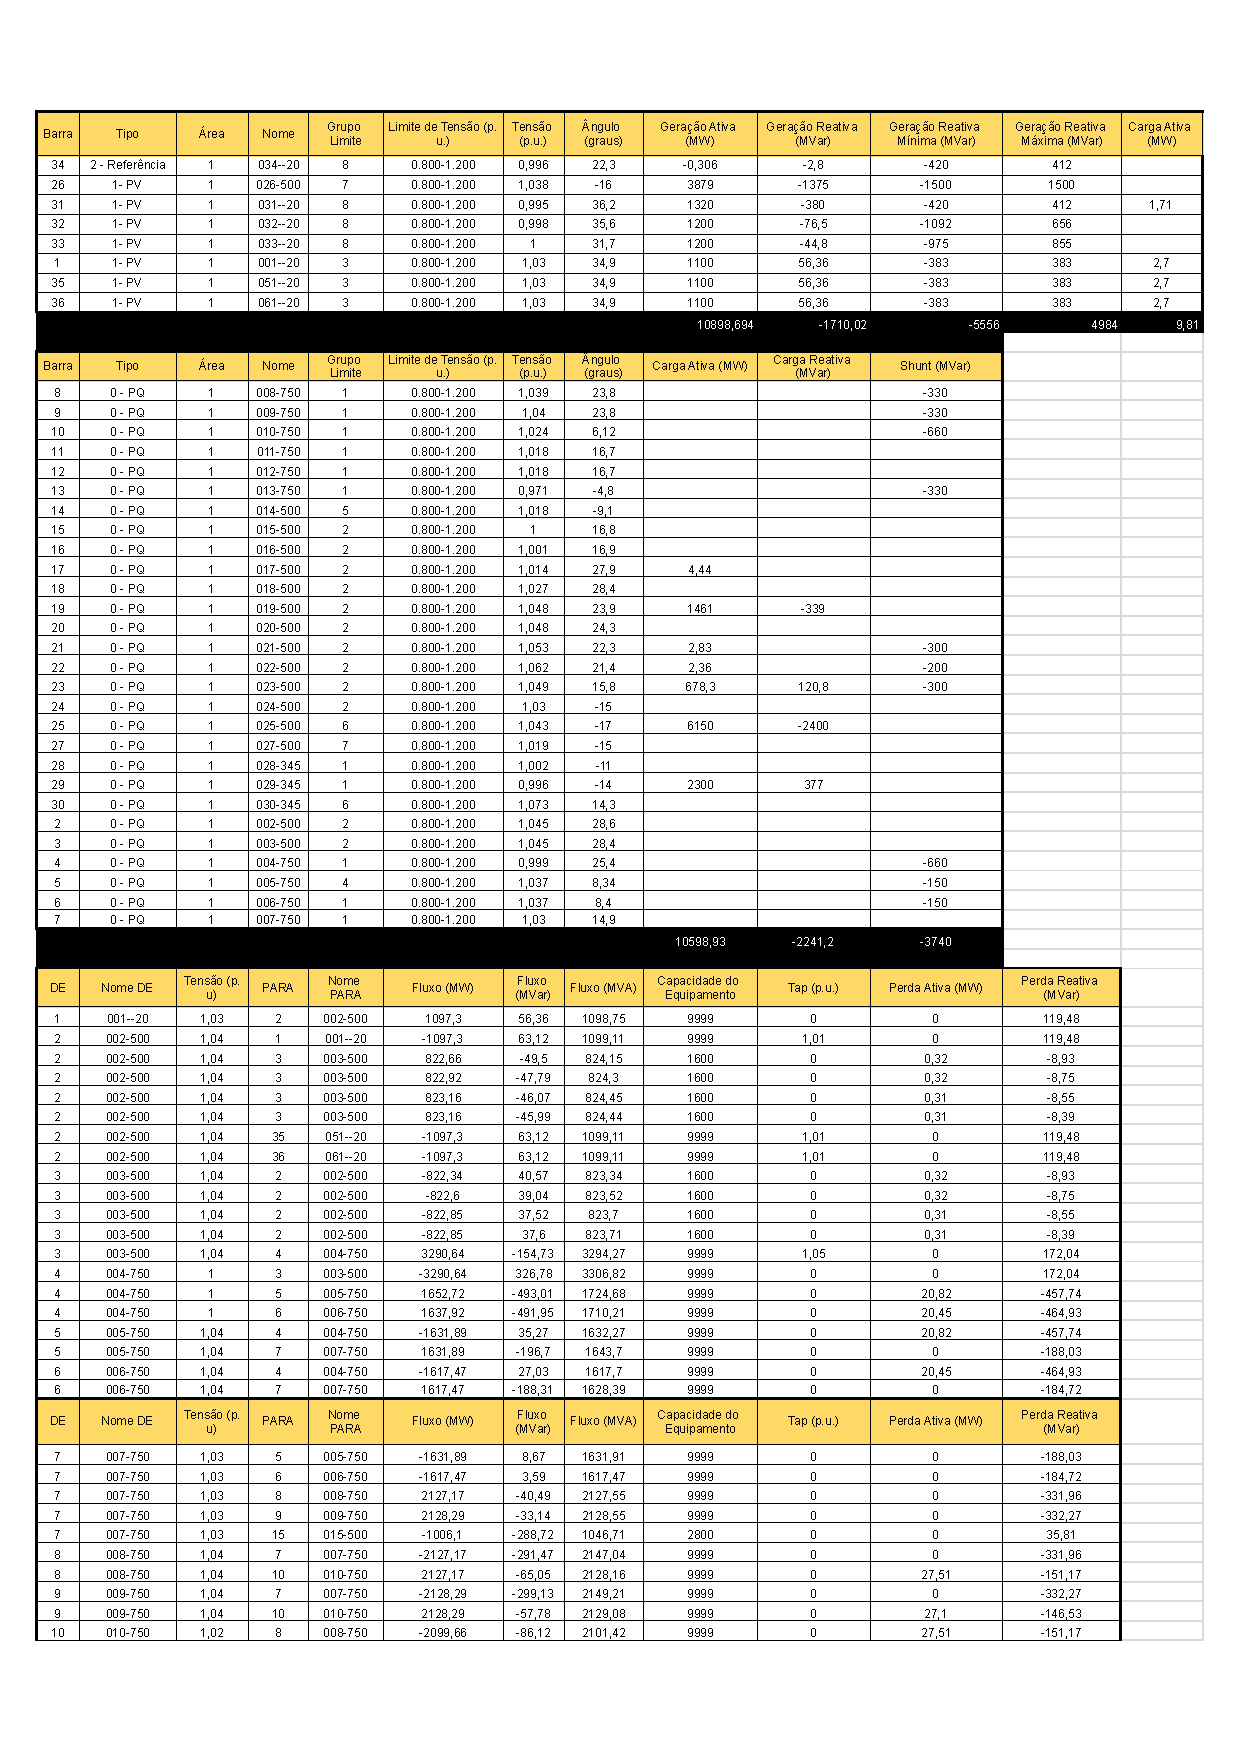
\includepdf[pages=-]{base_anarede.pdf}
	\par
	\chapter{Dados de Simulação do Anatem}
	\par
	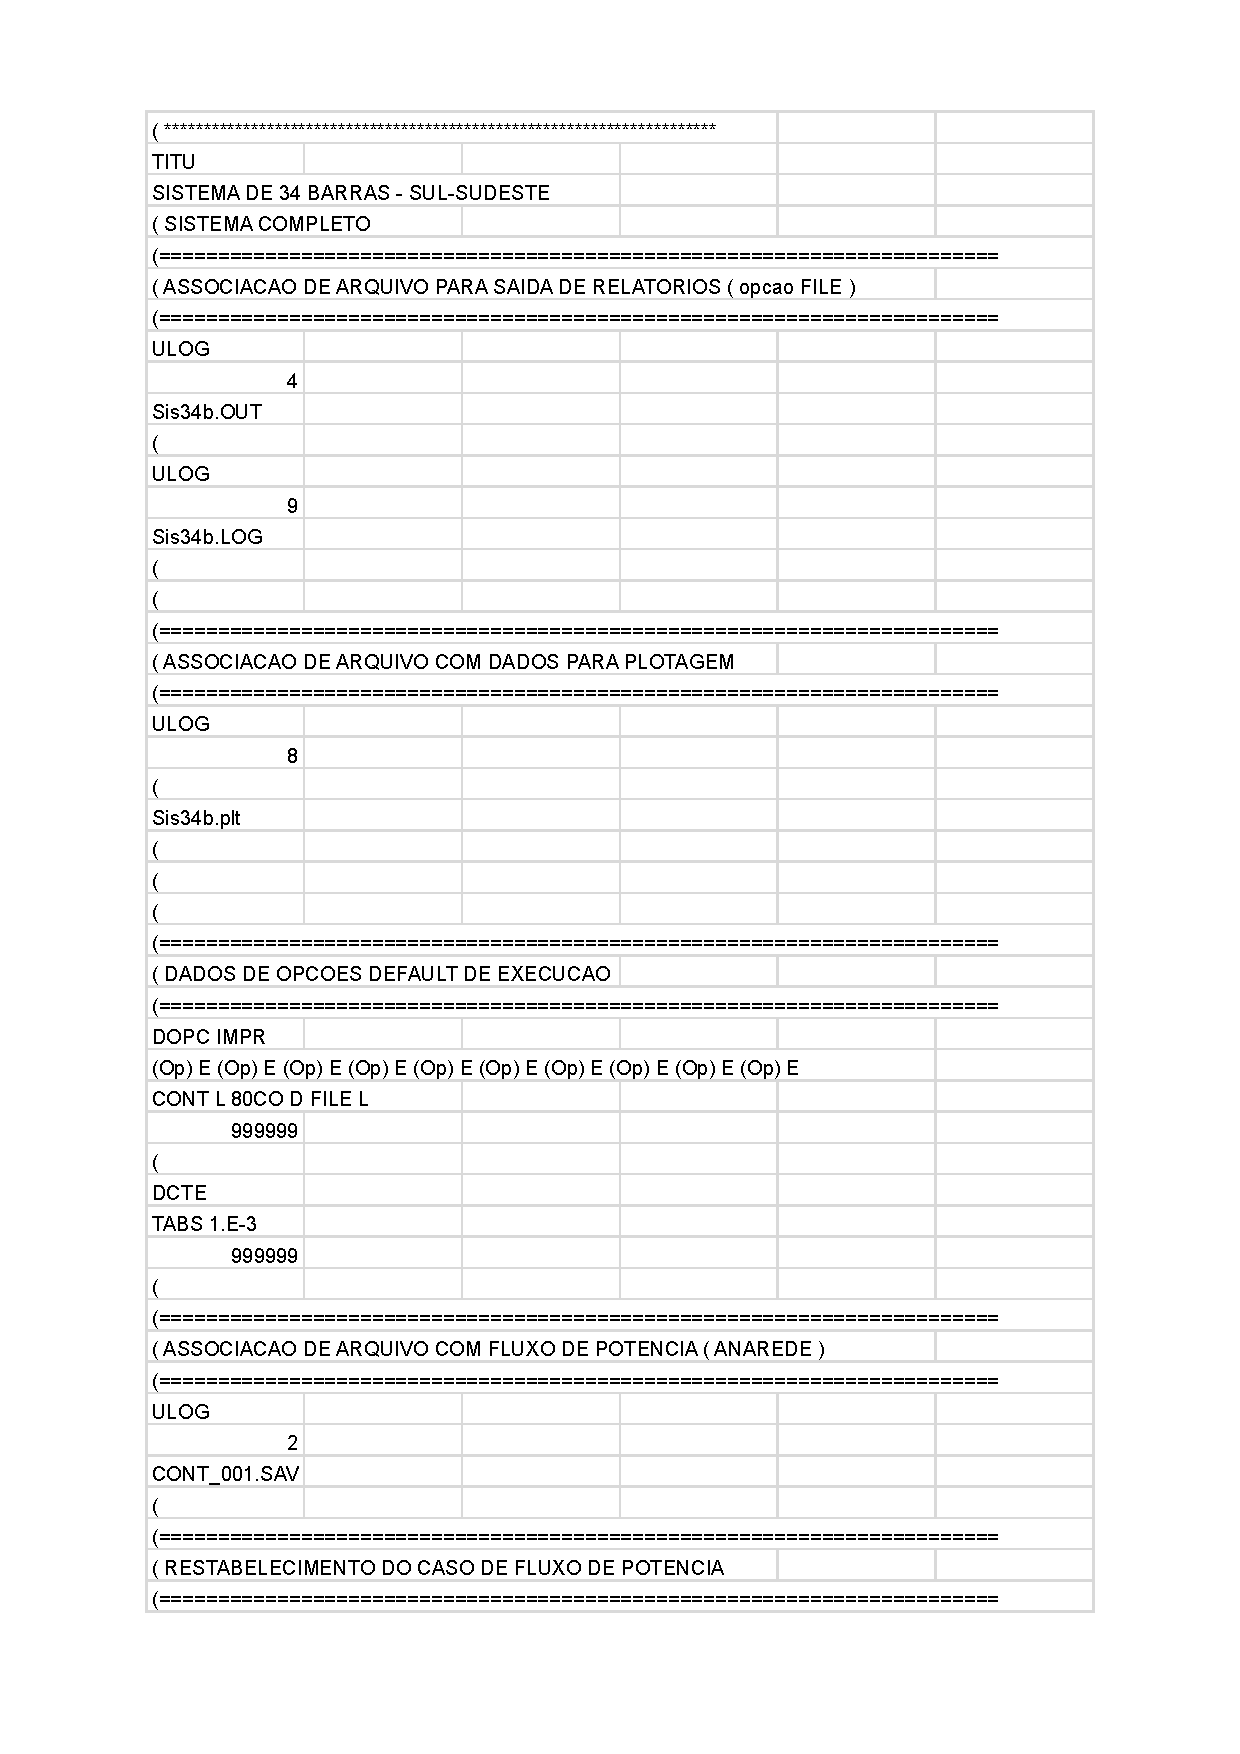
\includepdf[pages=-]{base_anatem.pdf}
	\par	
	\chapter{Modelos de Máquina e Curvas de Saturação}
	\par
	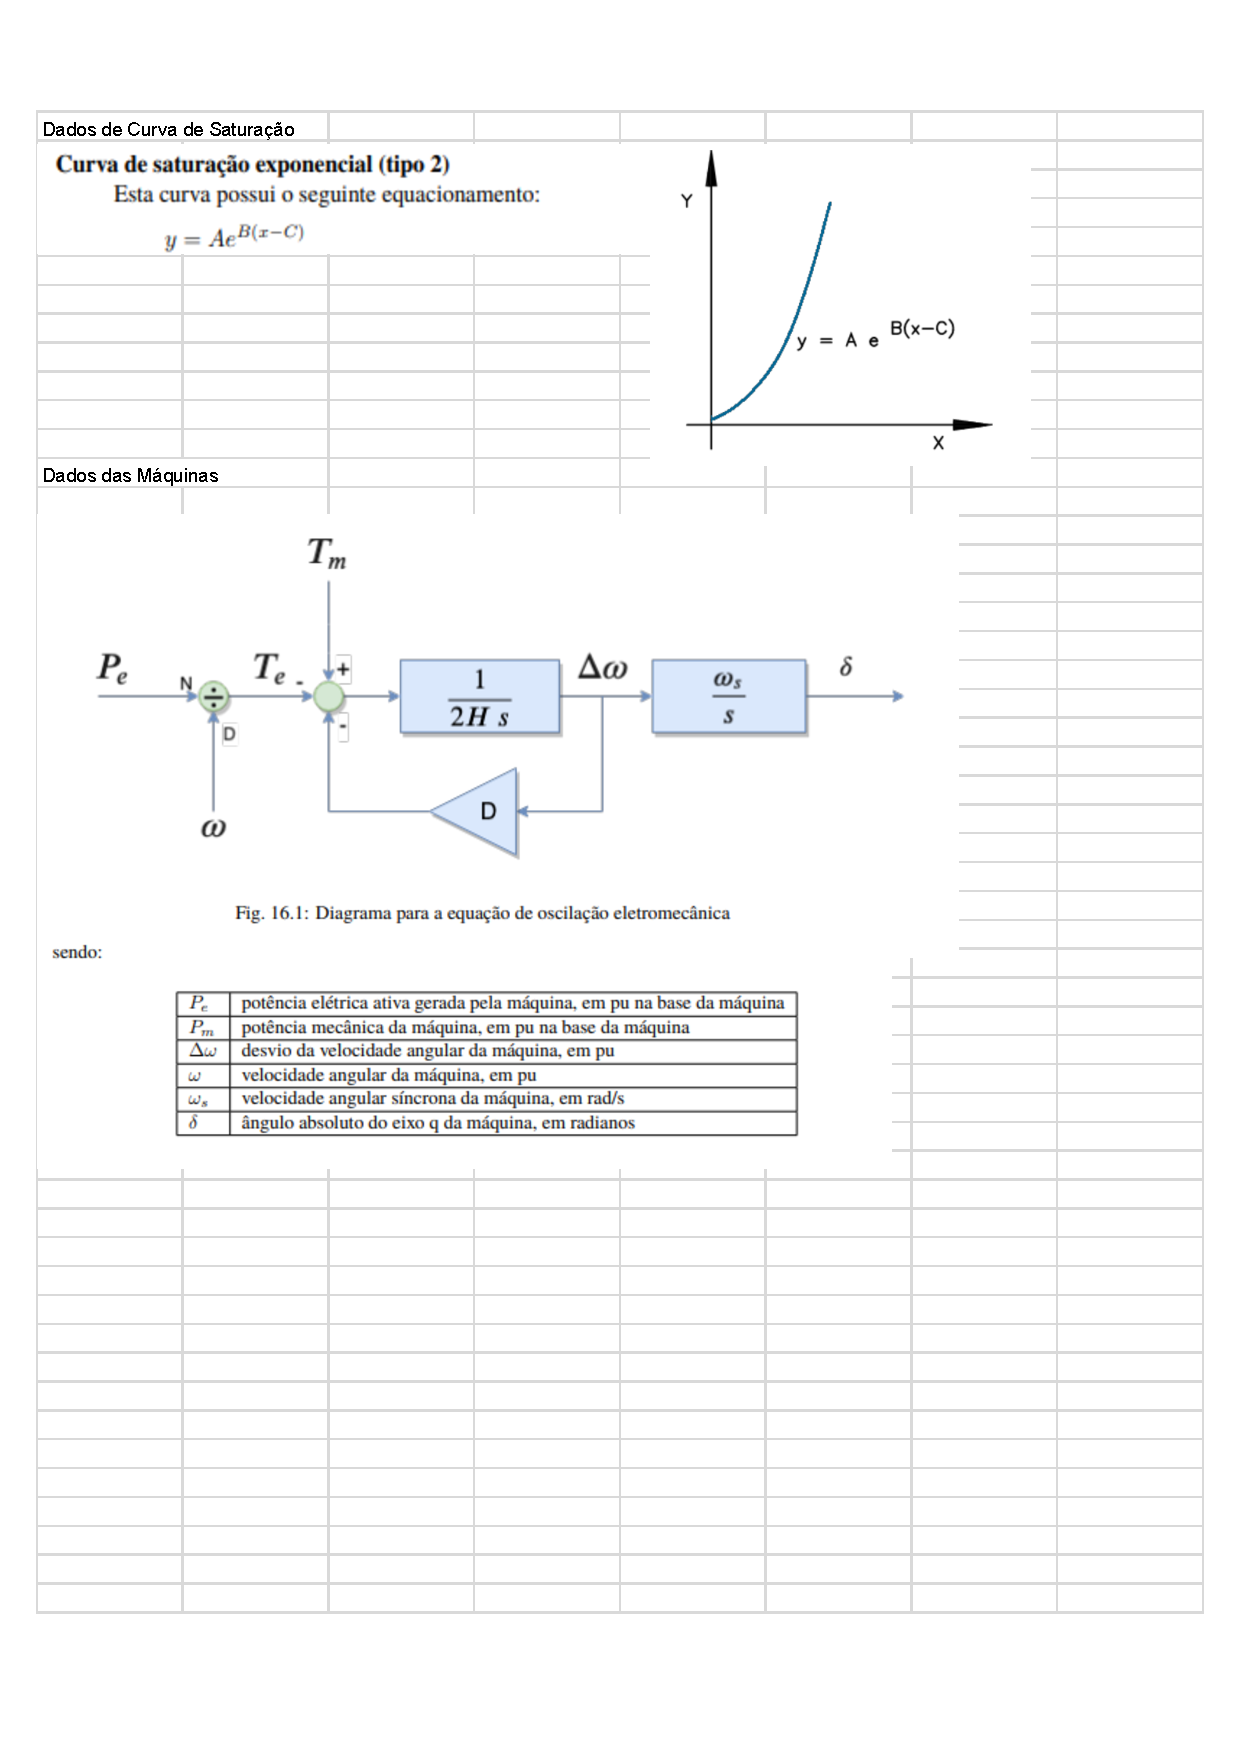
\includepdf[pages=-]{maquinas.pdf}
	\par	
	\chapter{Reguladores de Tensão e Velocidade}
	\par
	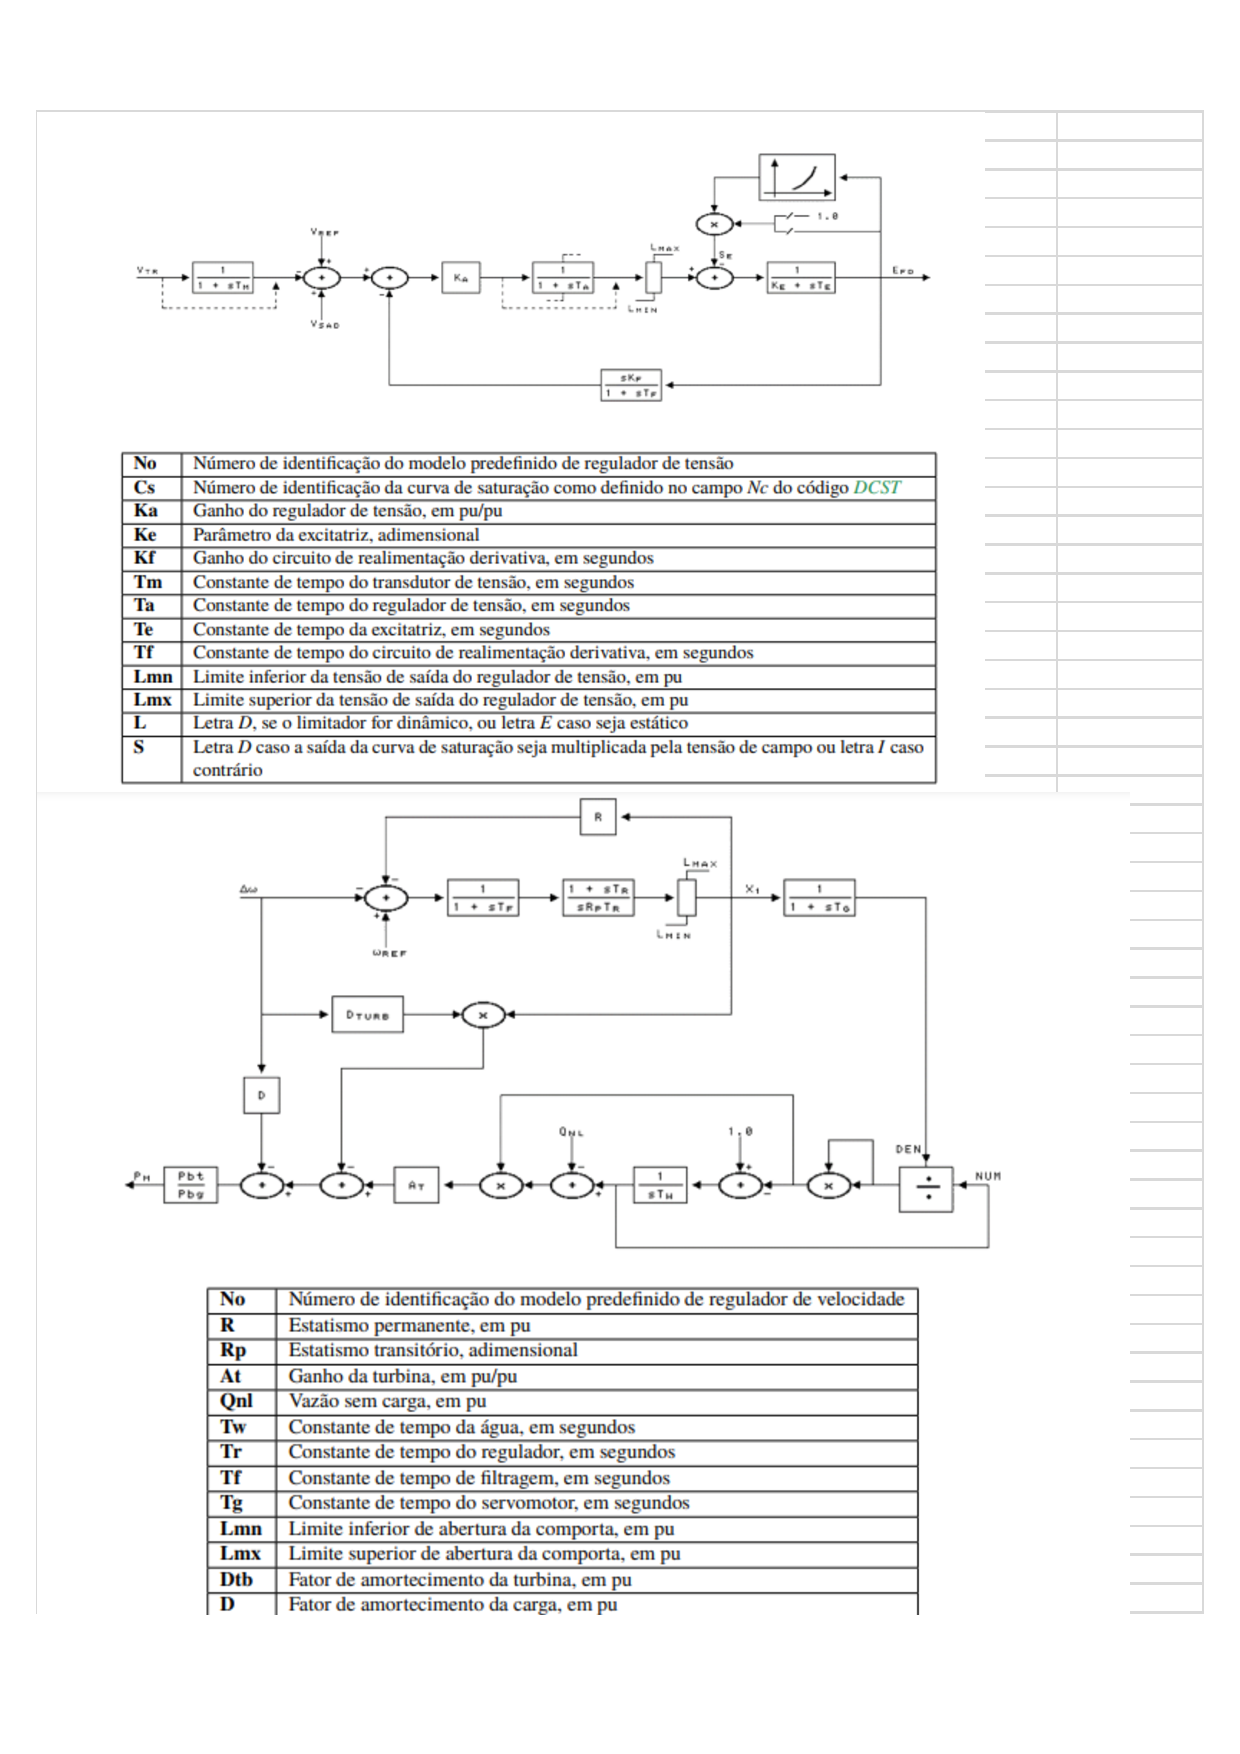
\includepdf[pages=-]{reguladores.pdf}
	\par	
	\chapter{Lista de Contingências Simuladas do Anatem}
	\par
	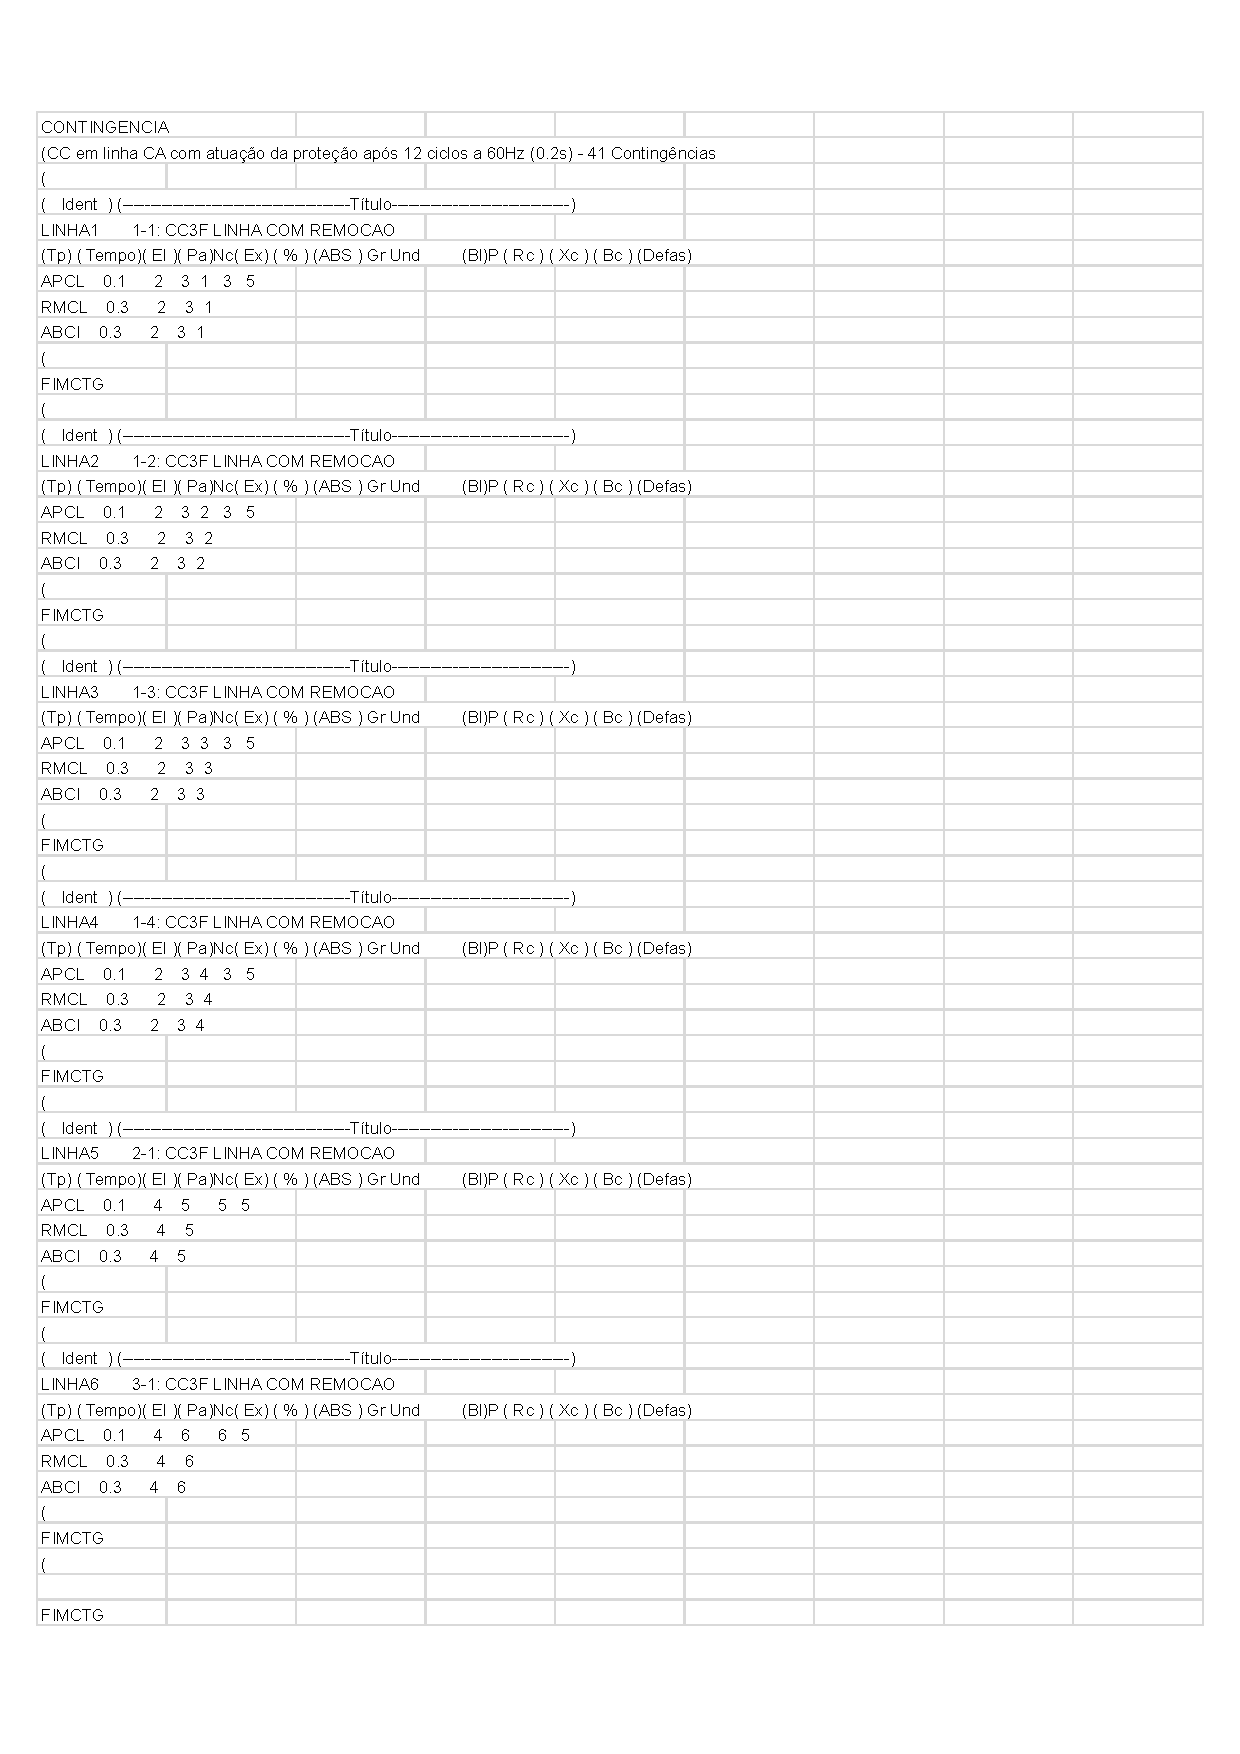
\includepdf[pages=-]{contingencias.pdf}
	\par	
	\chapter{Código em Python Utilizado}
	\par
	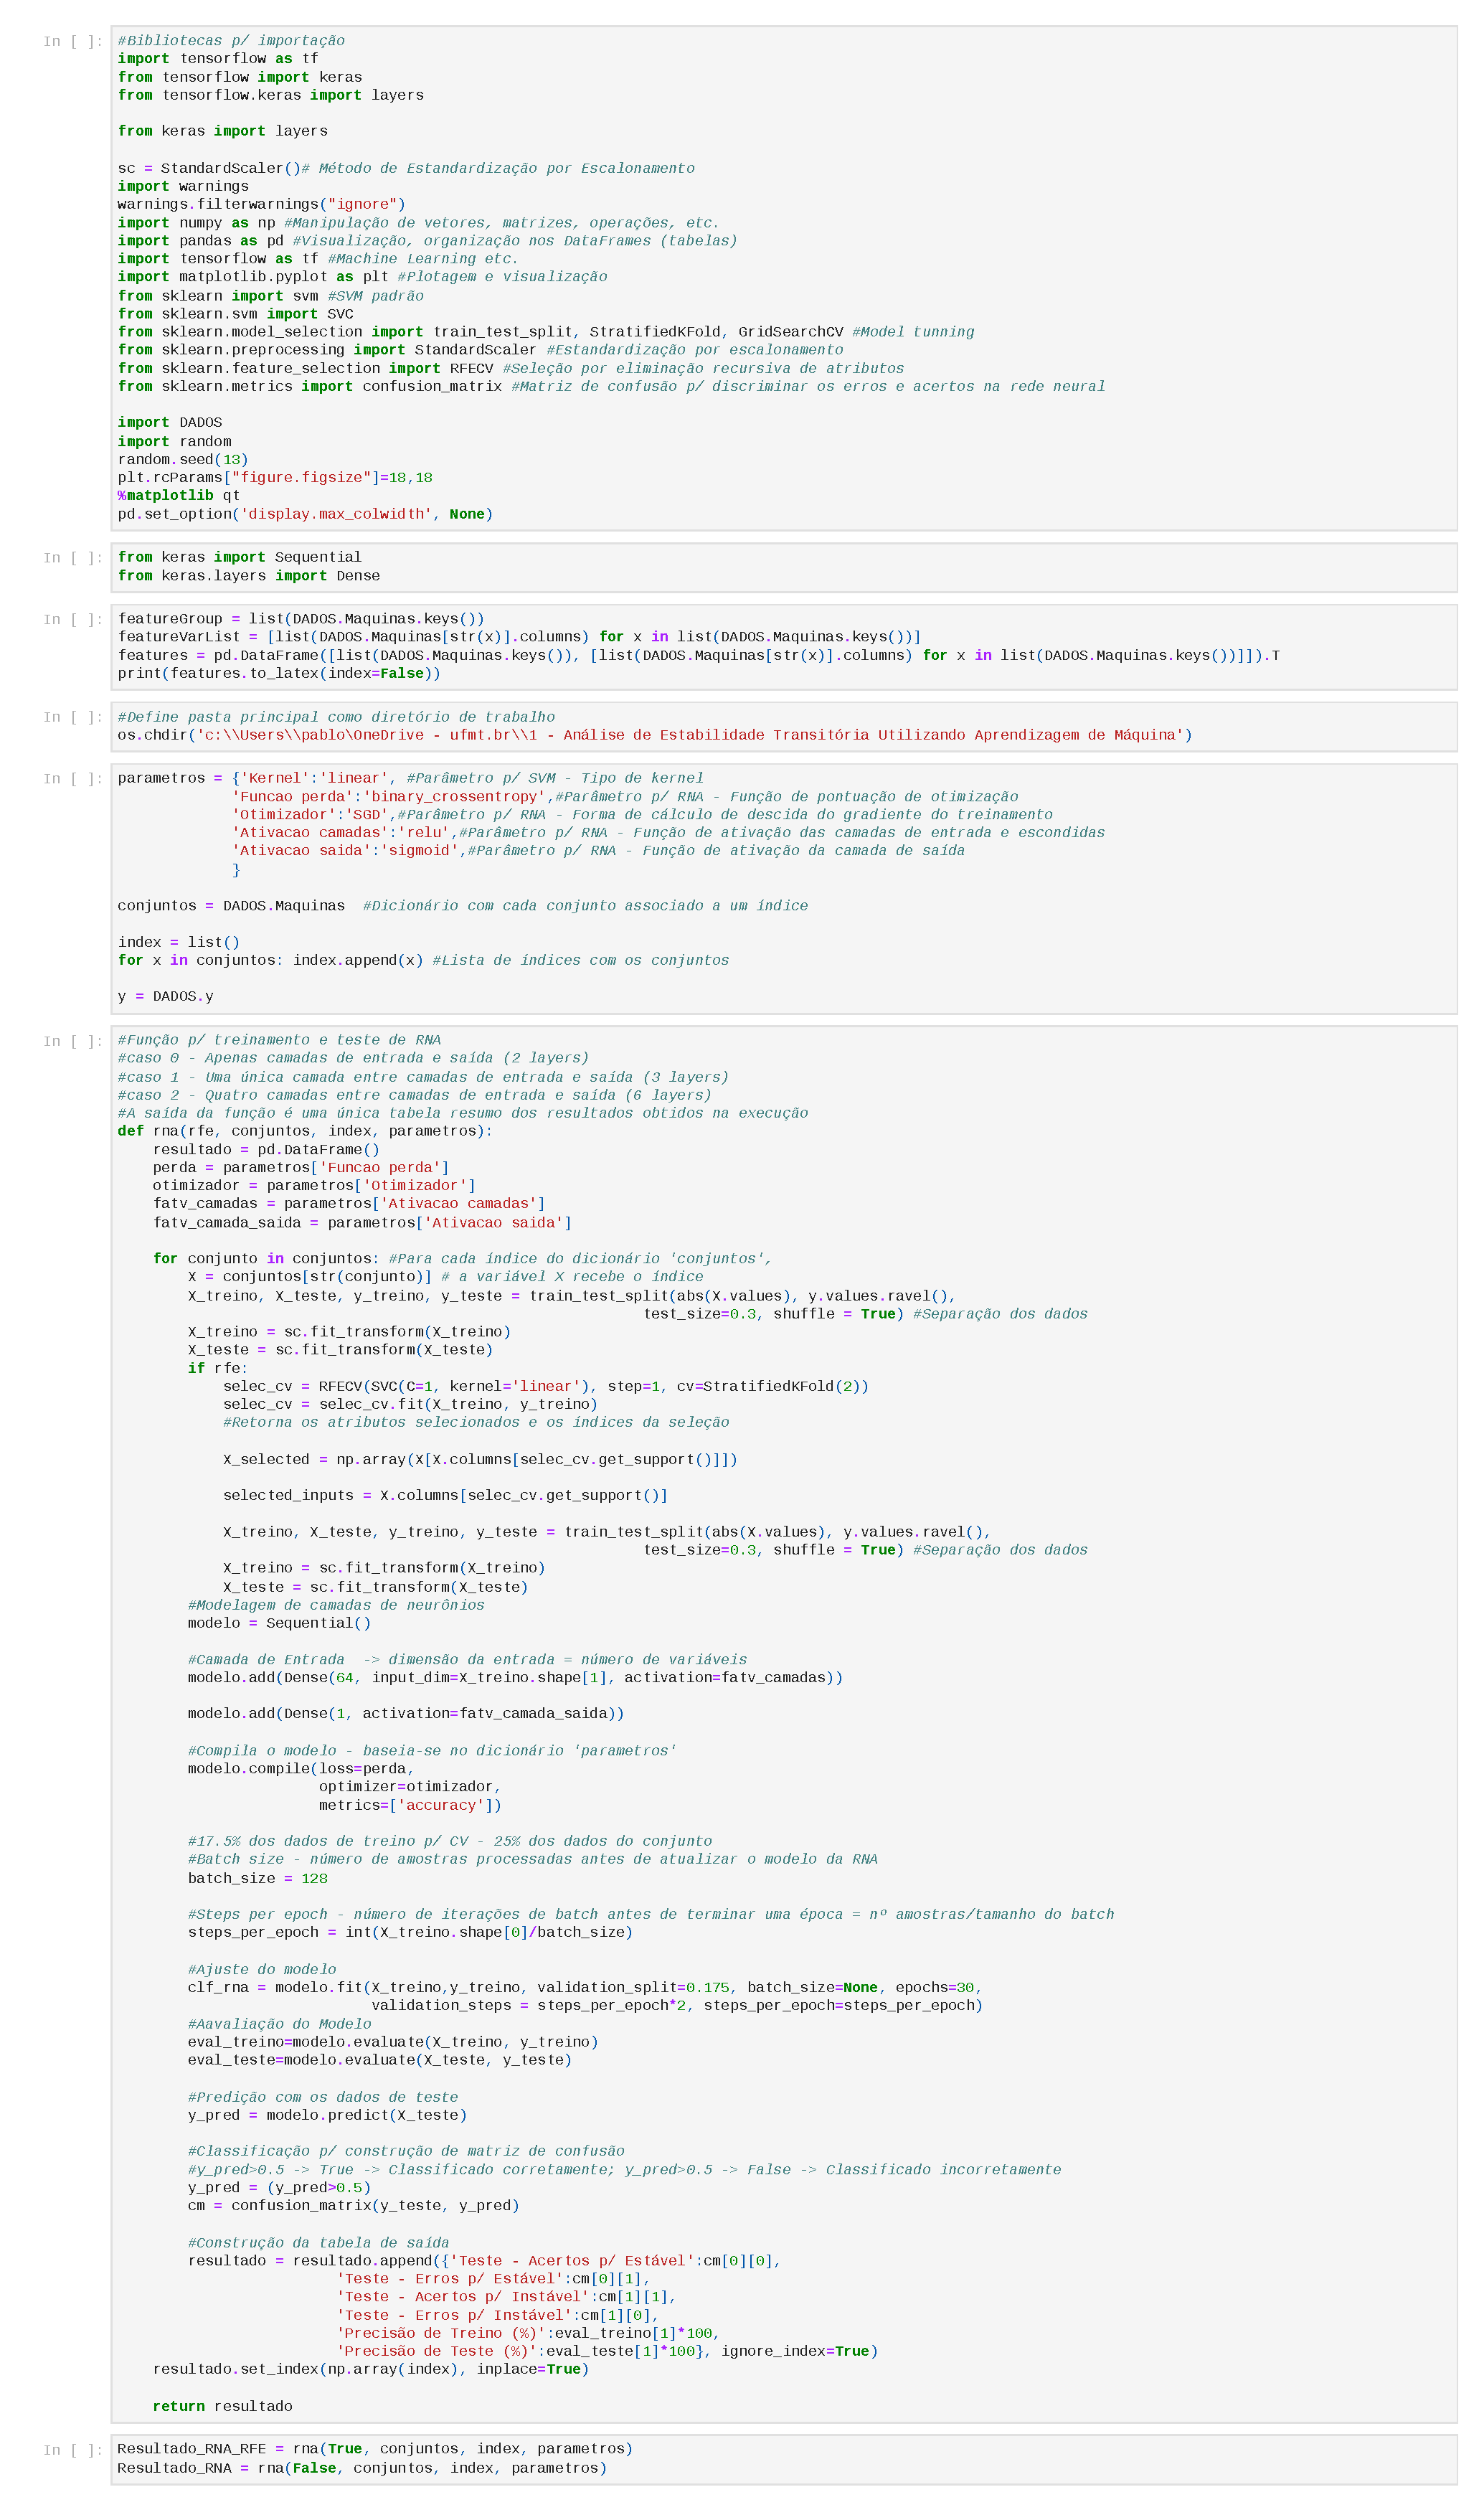
\includepdf[pages=-]{code_rna.pdf}
	\par	
	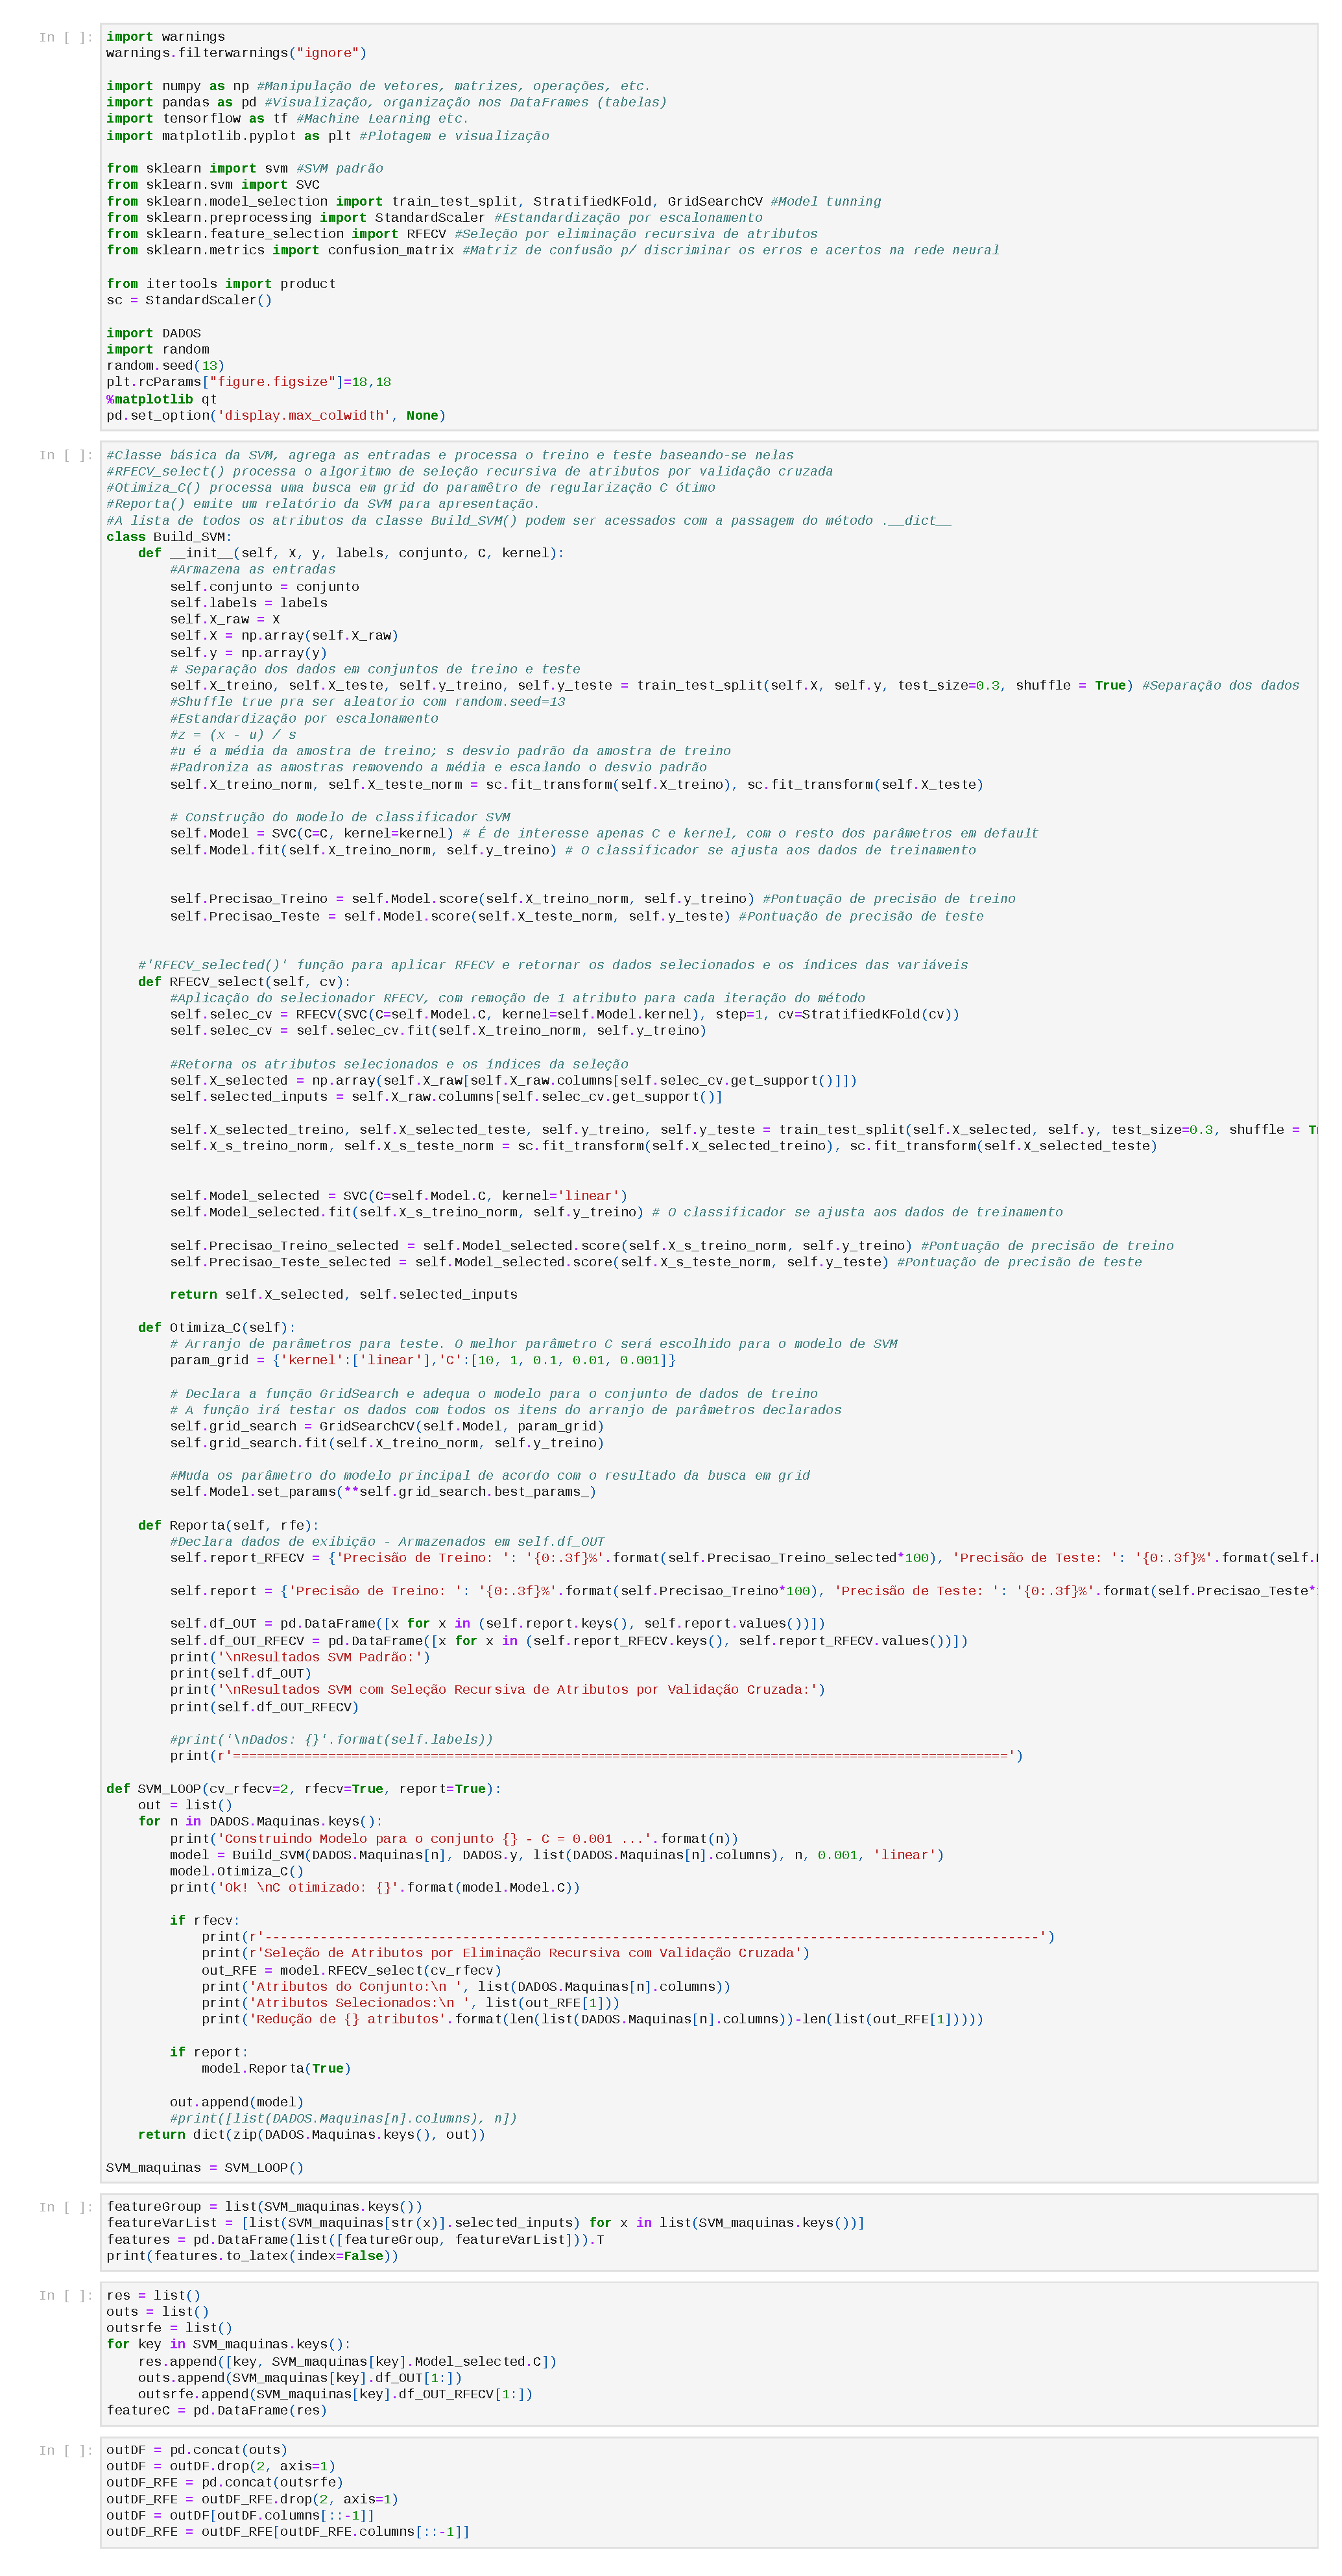
\includepdf[pages=-]{code_svm.pdf}
	\par
\end{apendicesenv}
	
	
\end{document}
